\documentclass[12pt,twoside,a4paper]{book}
\usepackage[pdftex]{graphicx}
\usepackage[pdftex]{hyperref}
\usepackage{a4}
\usepackage[margin=2cm]{geometry}
\pagestyle{headings}
% module description makros
\newcommand{\module}{\sf}
\newcommand{\modules}{\sf}
\newcommand{\sub}{\it}
\newcommand{\nam}{\it}
\newcommand{\modu}{\it}
\newcommand{\file}{\bf}
% miscellaneous
\newcommand{\e}[1]{\! \cdot \! 10^{#1}}
\newcommand{\plasim}{\bf Planet Simulator}
\newcommand{\most}{\bf Most16}
\newcommand{\model}{\bf Planet Simulator}
\newcommand{\modir}{plasim}
%%%%%%%%%%%%%%%%%%%%%%%%%%%

\begin{document}

\begin{titlepage}
\begin{figure}
\includegraphics[width=3cm]{Pics/uhhlogo}
{\textsf{\huge University of Hamburg}}
\end{figure}
\vspace*{1cm}
\begin{center}
{\Huge\bf \plasim} \\
\vspace*{1cm}
\includegraphics[width=13cm]{Pics/snaplasim} \\
\vspace*{1cm}
{\huge \bf User's Guide } \\
\vspace*{1cm}
{\huge \bf Version 16.0}
\vspace*{1cm}

 Frank Lunkeit   \\
 Simon Blessing  \\
 Klaus Fraedrich \\
 Heiko Jansen    \\
 Edilbert Kirk   \\ 
 Ute Luksch      \\
 Frank Sielmann  \\

\end{center}
\end{titlepage}

\begin{verbatim}
The Planet Simulator User's Guide is a publication of the
Theoretical Meteorology at the Meteorological Institute of
the University of Hamburg.

Address:

Prof. Dr. Klaus Fraedrich
Meteorological Institute
University of Hamburg
Bundesstrasse 55
D-20146 Hamburg

Contact:

Klaus.Fraedrich@zmaw.de
Frank.Lunkeit@zmaw.de
E.Kirk@gmx.de
\end{verbatim}

\tableofcontents

\chapter{Installation}
\chapter{Building and Installing}
\label{install} 
\lettrine{T}{his} chapter will walk through all aspects of EpiGrass installation. From obtaining, building and installing  the prerequisites to the installation of EpiGrass itself.

Most of the steps will be quite simple and similar since they will make use of standard tools for package installation on two very popular GNU/Linux distributions: Debian (and derivatives), and Gentoo. If you use a different distribution, you should check its documentation for package installation instructions.

If, on your distribution, a package is not available for the required version, you can try to obtain an updated version of the package at the web-sites provided. On the rare cases where pre-built packages are not available, instructions on how to build the software from source should also be available from its web-site.
\section{Required Packages}
\subsection{Python}
\begin{description}
\item[Web-site:] \url{http://www.python.org}
\item[Version required:] $\geq2.3$
\end{description}
Python is a simple but powerful object-orientated language. Its simplicity makes it easy to learn, but its power means that large and complex applications can be created. Its interpreted nature means that Python programmers are every productive because there is no edit/compile/link/run development cycle.

Python is probably installed automatically by your GNU/Linux distribution (it is on Gentoo). If not, it is best to use your distribution's standard tools for package installation. On Debian for example:
\begin{lstlisting}[frame=trBL, caption=Installation of Python in a Debian-based Gnu/Linux distribution. ,label=lst:pyinst]
$ apt-get install python
\end{lstlisting}

\subsection{Numeric Python}
\begin{description}
\item[Web-site:] \url{http://www.numpy.org}
\item[Version required:] $\geq23.0$
\end{description}
Numeric Python is a module for fast numeric computations in Python.

Example installations:
\begin{lstlisting}[frame=trBL, caption=Installing Numeric python on Gentoo GNU/Linux ,label=lst:instnumpyg]
$ emerge numeric
\end{lstlisting}
\begin{lstlisting}[frame=trBL, caption=Installing Numeric python on Debian GNU/Linux ,label=lst:instnumpyd]
$ apt-get install numeric
\end{lstlisting}

\subsection{Matplotlib}
\begin{description}
\item[Web-site:] \url{http://matplotlib.sourceforge.net}
\item[Version required:] $\geq0.70.0$
\end{description}
Matplotlib is a Module that provides plotting capabilities to Python.
\begin{lstlisting}[frame=trBL, caption=Installing Matplotlib on Gentoo GNU/Linux ,label=lst:instmplg]
$ emerge matplotlib
\end{lstlisting}
Before using \texttt{apt-get} to install matplotlib, add these lines to your  \texttt{/etc/apt/sources.list}:
\begin{lstlisting}[frame=trBL, caption=Adding specific sources to apt-get. ,label=]
deb http://anakonda.altervista.org/debian packages/
deb-src http://anakonda.altervista.org/debian sources/
\end{lstlisting}
\begin{lstlisting}[frame=trBL, caption=Installing Matplotlib on Debian GNU/Linux ,label=lst:instmpld]
$ apt-get update
$ apt-get install python-matplotlib python-matplotlib-doc
\end{lstlisting}


\subsection{Pygame}
\begin{description}
\item[Web-site:] \url{http://www.pygame.org}
\item[Version required:] $\geq1.6$
\end{description}
Pygame is a set of Python modules that wrap the excellent SDL library. Its the base of the EpiGrass OpenGL display.

Example installations:
\begin{lstlisting}[frame=trBL, caption=Installing Pygame python on Gentoo GNU/Linux ,label=lst:instpygameg]
$ emerge pygame
\end{lstlisting}
\begin{lstlisting}[frame=trBL, caption=Installing Pygame python on Debian GNU/Linux ,label=lst:instpygamed]
$ apt-get install pygame
\end{lstlisting}

\subsection{PyQt}
\begin{description}
\item[Web-site:] \url{http://www.riverbankcomputing.co.uk/pyqt/index.php}
\item[Version required:] $\geq3.13$
\end{description}
PyQt is a set of Python bindings for the Qt toolkit. PyQt combines all the advantages of Qt and Python. A programmer has all the power of Qt, but is able to exploit it with the simplicity of Python.

PyQt depends on the Qt libraries to run. This dependency will be taken care by the package installation tools of most distributions, which will automatically install the required version of Qt.

Example installations:
\begin{lstlisting}[frame=trBL, caption=Installing PyQt python on Gentoo GNU/Linux ,label=lst:instpyqtg]
$ emerge pyqt
\end{lstlisting}
\begin{lstlisting}[frame=trBL, caption=Installing PyQt python on Debian GNU/Linux ,label=lst:instpyqtd]
$ apt-get install python2.3-qt3
\end{lstlisting}
\subsection{MySQL}
\begin{description}
\item[Web-site:] \url{http://www.mysql.com}
\item[Version required:] $\geq4.0$
\end{description}
MySQL is a fast, multi-threaded, multi-user SQL database server. If you have a MySQL server available in your LAN, you may skip this step after making sure you have permission to access and use it to store your data.

Example installations:
\begin{lstlisting}[frame=trBL, caption=Installing MySQL on Gentoo GNU/Linux ,label=lst:instmysqlg]
$ emerge mysql
\end{lstlisting}
\begin{lstlisting}[frame=trBL, caption=Installing MySQL on Debian GNU/Linux ,label=lst:instmysqld]
$ apt-get install mysql-server
$ apt-get install mysql-client
\end{lstlisting}

\paragraph*{Post-install configuration:}
MySQL requires a few extra configuration steps that must be completed after the installation described above. These steps must be performed by the root user.
\begin{lstlisting}[frame=trBL, caption=Post-install configuration of mysql on Gentoo ,label=lst:mysqlconfg]
$ /etc/init.d/mysql start
$ mysql_install_db
$ mysqladmin -u root password new-password
$ rc-update add mysql default
\end{lstlisting}
In the mysqladmin line, replace new-password with a password of your own. 

\begin{lstlisting}[frame=trBL, caption=Post-install configuration of mysql on Debian ,label=lst:mysqlconfd]
$ mysql_install_db
$ safe_mysqld &
$ /etc/init.d/mysql start
$ mysqladmin -u root password new-password
\end{lstlisting}

\subsection{MySQL-python}
\begin{description}
\item[Web-site:] \url{http://sourceforge.net/projects/mysql-python/}
\item[Version required:] $\geq0.9.2$
\end{description}
This package is a MySQL module for Python.

Example installations:
\begin{lstlisting}[frame=trBL, caption=Installing MySQL-python on Gentoo GNU/Linux ,label=lst:instmysqlpyg]
$ emerge mysql-python
\end{lstlisting}
\begin{lstlisting}[frame=trBL, caption=Installing MySQL-python  on Debian GNU/Linux ,label=lst:instmysqlpyd]
$ apt-get install python2.3-mysqldb
\end{lstlisting}
\subsection{R}
\begin{description}
\item[Web-site:] \url{http://www.r-project.org}
\item[Version required:] $\geq2.0$
\end{description}
Example installations:
\begin{lstlisting}[frame=trBL, caption=Installing R on Gentoo GNU/Linux ,label=lst:instRg]
$ emerge R
\end{lstlisting}
\begin{lstlisting}[frame=trBL, caption=Installing R on Debian GNU/Linux ,label=lst:instRd]
$ apt-get install r-base
\end{lstlisting}
\paragraph*{Post-install configuration:}
You have to install a few packages from within R afterward.
\begin{lstlisting}[frame=trBL, caption=Installing aditional packages from within R ,label=lst:instRpkgs]
> install.packages('RMySQL')
> install.packages('DBI')
> install.packages('lattice')
\end{lstlisting}

\subsection{RPy}
\begin{description}
\item[Web-site:] \url{http://rpy.sourceforge.net/}
\item[Version required:] $\geq0.4.0$
\end{description}
RPy is a very simple, yet robust, Python interface to the R Programming Language. It can manage all kinds of R objects and can execute arbitrary R functions (including the graphic functions). 
Example installations:
\begin{lstlisting}[frame=trBL, caption=Installing RPy on Gentoo GNU/Linux ,label=lst:instRPyg]
$ emerge rpy
\end{lstlisting}
If the \texttt{rpy} package on Gentoo is masked\footnote{Meaning that it can't be installed normally.}, use the method described for installing on Debian, below. 

On Debian download the RPy source tarball, unpack it, \texttt{cd} to the directory to which you unpacked it and type:
\begin{lstlisting}[frame=trBL, caption=Installing RPy on Debian GNU/Linux ,label=lst:instRPyd]
$ python setup.py install
\end{lstlisting}
RPy depends on R having been compiled with the option \texttt{--enable-R-shlib}. This is the default on Gentoo. If this installation fails on your system, you may have to get the latest version from rpy from its website and install from source by following these steps:
\begin{enumerate}
\item First of all, you \textbf{must} check that you have built R with the configure
    option '--enable-R-shlib', in order to make R as a shared library.  If
    not, the following steps should be enough:
\begin{lstlisting}[frame=trBL, caption=Building R from source ,label=lst:rfs]
 <go to the R source directory>
$ make distclean
$ ./configure --enable-R-shlib
$ make
$ sudo make install
\end{lstlisting}
 


\item Then, configure the path to the R library. For this, make a link to RHOME/bin/libR.so in /usr/local/lib or /usr/lib, then run \texttt{ldconfig},  (substitute RHOME with the path where R is installed, usually
    \/usr\/local\/lib\/R):
\begin{lstlisting}[basicstyle=\footnotesize,frame=trBL, caption= ,label=]
$ sudo ln -s /usr/local/lib/R/lib/libR.so /usr/lib/libR.so
\end{lstlisting}

\item Ensure that you have the necessary header files for the version of R you are 
    compiling against.  You can check the version of R by running:
\begin{lstlisting}[frame=trBL, caption= ,label=]
$ R --version
R 2.0.1 (2004-11-15).
Copyright (C) 2004 R Development Core Team

R is free software and comes with
ABSOLUTELY NO WARRANTY.
You are welcome to redistribute it under 
the terms of the GNU General Public License.  
For more information about these matters,
see http://www.gnu.org/copyleft/gpl.html.
\end{lstlisting}


    There should be a subdirectory of the Rpy package with the name
\texttt{R-<version>}.For the example above, \texttt{R-2.0.1}

    If the correct version directory does not exist, you may have to go back to a version of \texttt{R} supported by rpy.


\item Now, just type:
\begin{lstlisting}[frame=trBL, caption= ,label=]
$ python setup.py install
\end{lstlisting}
       

    and that's all!

\end{enumerate}



\subsection{Grass GIS}
\begin{description}
\item[Web-site:] \url{http://grass.itc.it/}
\item[Version required:] $\geq5.0.3$
\end{description}
\begin{lstlisting}[frame=trBL, caption=Installing GRASS on Gentoo GNU/Linux ,label=lst:instgrassg]
$ emerge grass
\end{lstlisting}

\begin{lstlisting}[frame=trBL, caption=Installing GRASS on Debian GNU/Linux ,label=lst:instgrassd]
$ apt-get install grass
\end{lstlisting}

\subsection{\LaTeX}
\begin{description}
\item[Web-site:] \url{http://www.tug.org/teTeX/}
\item[Version required:] $\geq2.0$
\end{description}
EpiGrass uses \LaTeX  or PDF\LaTeX  to generate a report with a summary analysis of your network and simulation model. Thus, it is necessary to have the Tetex package installed.
\begin{lstlisting}[frame=trBL, caption=Installing \LaTeX and PDF\LaTeX on Gentoo GNU/Linux ,label=lst:insttexg]
$ emerge tetex
\end{lstlisting}

\begin{lstlisting}[frame=trBL, caption=Installing \LaTeX and PDF\LaTeX on Debian GNU/Linux ,label=lst:insttexd]
$ apt-get install tetex-base
\end{lstlisting}

\section{Installing EpiGrass}
If you got through all the steps above, it will be an easy task to install EpiGrass:
\begin{lstlisting}[frame=trBL, caption=Intalling EpiGrass ,label=lst:instepg]
$ python setup.py install
\end{lstlisting}

We have written an ebuild for installing epigrass on Gentoo. If it is unmasked at the time you decide to install epigrass, you don't need to worry about the dependencies above and only need to type the following command:
\begin{lstlisting}[frame=trBL, caption=Installing EpiGrass on Gentoo GNU/Linux ,label=lst:instepgg]
$ emerge epigrass
\end{lstlisting}

\chapter{Modules}
This is a technical documentation of the PUMA-II model. In the following, the purposes of the
individual modules is given and the general structure and possible input and output
opportunities
(namelist, files) are explained. 

%------------------------------------------------------------------------

% \clearpage
\begin{center}
\begin{tabular}{|p{14cm}|}
\hline
\vspace{-5mm} \section{fluxmod.f90} \vspace{-5mm} \\
\hline
\vspace{1mm} {\bf General} The module {\module fluxmod.f90} contains subroutines to
compute the different surface fluxes and to perform the vertical diffusion. The interface to the
main PUMA module {\module puma.f90} is given by the subroutines {\sub fluxini}, {\sub
fluxstep} and {\sub fluxstop} which are called in {\module puma.f90} from the subroutines
{\sub prolog}, {\sub gridpointd} and {\sub epilog}, respectively. \vspace{3mm} \\
\hline
\vspace{1mm} {\bf Input/Output} {\module fluxmod.f90} does not use any extra input file  or
output file and  is controlled by the namelist {\nam fluxpar} which is part of the namelist file
{\file puma$\_$namelist}:

 \vspace{1mm} 

\begin{center}
\begin{tabular}{l l p{7cm} c}  %  {p{3cm} p{2cm} p{6cm} p{2cm}}
Parameter & Type & Purpose & Default \\
&&&\\
NEVAP & Integer & Switch for surface evaporation (0~=~off, 1~=~ on) & 1 \\
NSHFL & Integer &Switch for surface sensible heat flux (0~=~off, 1~=~ on) & 1 \\
NSTRESS & Integer & Switch for surface wind stress (0~=~off, 1~=~on) & 1 \\
NTSA & Integer & Switch for computing the near surface air temperature which is used for the
Richardson number (1~=~potential temperature, 2~=~virtual potential temperature)& 2 \\
NVDIFF & Integer & Switch for vertical diffusion (0~=~off, 1~=~on) & 1 \\
VDIFF$\_$LAMM & Real & Tuning parameter for vertical diffusion & 160. \\
VDIFF$\_$B & Real &Tuning parameter for vertical diffusion & 5. \\
VDIFF$\_$C & Real &Tuning parameter for vertical diffusion & 5. \\
VDIFF$\_$D & Real &Tuning parameter for vertical diffusion & 5. \\
\end{tabular} 
\end{center}
\vspace{3mm} \\
\hline
\vspace{2mm} {\bf Structure} Internally, {\module fluxmod.f90} uses the FORTRAN-90
module {\modu fluxmod}, which uses the global common module {\modu pumamod} from
{\module pumamod.f90}. Subroutine {\sub fluxini} reads the namelist and, if the parallel
version
is used,  distributes the namelist parameters to the different processes. Subroutine {\sub
fluxstep}
calls the subroutine {\sub surflx} to compute the surface fluxes and calls the subroutine {\sub
vdiff} to do the vertical diffusion. Subroutine {\sub fluxstop} is a dummy subroutine since there
is nothing to do to finalize the computations in {\module fluxmod.f90}. The computation of the
surface fluxes in {\sub surflx} is spitted into several parts. After initializing the stability
dependent transfer coefficients, the subroutines {\sub mkstress}, {\sub mkshfl} and {\sub
mkevap} do the computations which are related to the surface wind stress, the surface sensible
heat flux and the surface evaporation, respectively. \vspace{3mm} \\
\hline
\end{tabular}
\end{center}
\newpage
%--------------------------------------------------------------------------------

\begin{center}
\begin{tabular}{|p{14cm}|}
\hline
\vspace{-5mm} \section{miscmod.f90} \vspace{-5mm} \\
\hline
\vspace{1mm} {\bf General} The module {\module miscmod.f90} contains miscellaneous
subroutines which do not fit well to other modules. The interface to the main PUMA module
{\module puma.f90} is given by the subroutines {\sub miscini}, {\sub miscstep} and {\sub
miscstop} which are called in {\module puma.f90} from the subroutines {\sub prolog}, {\sub
gridpointd} and {\sub epilog}, respectively. A subroutine to eliminate spurious negative
humidity and an optional subroutine to relax the upper level temperature towards a prescribed 
distribution is included in {\module miscmod.f90}. \vspace{3mm} \\
\hline
\vspace{1mm} {\bf Input/Output} {\module miscmod.f90}  does not use any extra output file.
If the relaxation is switched on, a climatological annual cycle of the prescribed  upper level
temperature distribution [K] is read from the external file {\file CLIMATEFILE} (see namelist).
The file format is formatted SERVICE format with (8I10) for the headers and (8E12.6) for the
temperature fields. To assign the field, the header needs to have the header information code
130,
level 1 and a date identifier of the form {\it yymmdd} or {\it mmdd} where {\it mm} goes from
01 to 12 (January to December). Fields which are not needed will be skipped. The module is
controlled by the namelist {\nam miscpar} which is part of the namelist file {\file
puma$\_$namelist}:

\vspace{1mm} 

\begin{center}
\begin{tabular}{l l p{5cm} c} % {p{3cm} p{2cm} p{6cm} p{2cm}}
Parameter & Type & Purpose & default \\
&&& \\
NFIXER & Integer & Switch for correction of negative moisture (0 = off , 1= on) & 1 \\
NUDGE  & Integer & Switch for temperature relaxation in the uppermost level (0 = off , 1= on)
& 0 \\
TNUDGE& Real & Time scale [d] of the temperature relaxation & 10. \\
CLIMATEFILE& Character & Name of the file containing the prescribed temperature
distribution & surface\underline{ }parameter  
\end{tabular} 
\end{center}
\vspace{3mm} \\
\hline
\vspace{2mm} {\bf Structure} Internally, {\module miscmod.f90} uses the FORTRAN-90
module {\modu miscmod}, which uses the global common module {\modu pumamod} from
{\module pumamod.f90}. Subroutine {\sub miscini} reads the namelist and, if the parallel
version is used,  distributes the namelist parameters to the different processes. If the relaxation
is
switched on, the climatological temperature is read from {\file CLIMATEFILE} and distributed
to the processors.   Subroutine {\sub miscstep} calls the subroutine {\sub fixer} to eliminate
spurious negative humidity arising from the spectral method and, if the relaxation is switched
on,
calls the subroutine {\sub mknudge} to do the temperature nudging. Subroutine {\sub miscstop}
is a dummy subroutine since there is nothing to do to finalize the computations in {\module
miscmod.f90}. \vspace{3mm} \\
\hline
\end{tabular}
\end{center} 
\newpage
%--------------------------------------------------------------------------------
\clearpage
\begin{center}
\begin{tabular}{|p{14cm}|}
\hline
\vspace{-5mm} \section{surfmod.f90} \vspace{-5mm} \\
\hline
\vspace{1mm} {\bf General} The module {\module surfmod.f90} deals as an interface between
the atmospheric part of the model and modules, or models, for the land and the oceans. The
interface to the main PUMA module {\module puma.f90} is given by the subroutines {\sub
surfini}, {\sub surfstep} and {\sub surfstop} which are called in {\module puma.f90} from the
subroutines {\sub prolog}, {\sub gridpointd} and {\sub epilog}, respectively. Calls to
subroutines
named {\sub landini}, {\sub landstep} and {\sub landstop} and {\sub seaini}, {\sub seastep} and
{\sub seastop} provide the interface to land and the ocean modules, respectively.
\vspace{3mm}
\\
\hline
\vspace{1mm} {\bf Input/Output} {\module surfmod.f90} reads the land-sea mask [frac.] and
the orography (surface geopotential) [m$^2$/s$^2$] from file {\file INPUTFILE} (see
namelist). 
The file format is formatted SERVICE format with (8I10) for the headers and (8E12.6) for the
fields. To
assign
the fields, the headers need to have the header information code 129 for the surface geopotential
and 172 for the land-sea  mask (1. = land; 0. = sea). Fields which are not needed will be skipped. 
{\module surfmod.f90} is controlled by the namelist {\nam surfpar} which is part of the
namelist file {\file puma$\_$namelist}:

\vspace{1mm} 

\begin{center}
\begin{tabular}{l l p{5cm} c} %{p{3cm} p{2cm} p{6cm} p{2cm}}
Parameter & Type & Purpose & default \\
&&&\\
NSURF & Integer & Debug switch  & not active \\
NOROMAX & Integer & Resolution of orography & NTRU \\
OROSCALE & Real & Scaling factor for orography & 1.0 \\
INPUTFILE& Character & Name of the input file & surface\underline{ }parameter  
\end{tabular} 
\end{center}
\vspace{3mm} \\
\hline
\vspace{2mm} {\bf Structure} Internally, {\module surfmod.f90} uses the FORTRAN-90
module {\modu surfmod}, which uses the global common module {\modu pumamod} from
{\module pumamod.f90}. Subroutine {\sub surfini} reads the namelist and, if the parallel
version
is used,  distributes the namelist parameters to the different processes. If the run is not started
from a restart file (NRESTART from namelist {\nam inp}of {\module puma.f90} is 0), the
land-sea-mask and the
orography are read from file {\file INPUTFILE}. According to the namelist input, the
orography
is scaled by OROSCALE, transfered into spectral space and truncated to NOROMAX. Calls to
subroutines {\sub landini} and {\sub seaini} are the interfaces to the respective initialization
routines contained in the land and ocean modules. During the run, the interface to land and
ocean
is given by calls to the external subroutines {\sub landstep} and {\sub seastep}, which are called
by {\sub surfstep}. At the end of the integration, interface subroutines {\sub landstop} and {\sub
seastop} are called by {\sub surfstop}. \vspace{3mm} \\
\hline
\end{tabular}
\end{center} 
\newpage
%--------------------------------------------------------------------------------

\begin{center}
\begin{tabular}{|p{14cm}|}
\hline
\vspace{-5mm} \section{fftmod.f90} \vspace{-5mm} \\
\hline
\vspace{1mm} {\bf General} The module {\module fftmod.f90} contains all subroutines
necessary to perform the fast fourier transformation and its inverse. The interface to the main
PUMA module {\module puma.f90} and to other modules (at the moment {\module
surfmod.f90}, {\module
legmod.f90} and {\module rainmod.f90}) is given by the subroutines {\sub gp2fc} and {\sub
fc2gp} which are called in {\module puma.f90} from the subroutines {\sub gridpointa} and
{\sub gridpointd}, in {\module surfmod.f90} from {\sub surfini}, in {\module legmod.f90}
from {\sub sp2gp}, and in {\module rainmod.f90} from {\sub mkdqdtgp}.  \vspace{3mm} \\
\hline
\vspace{1mm} {\bf Input/Output} {\module fftmod.f90} does not use any extra input file or
output file. No namelist input is required. \vspace{3mm} \\
\hline
\vspace{2mm} {\bf Structure} Internally, {\module fftmod.f90} uses the FORTRAN-90 module
{\modu fftmod}, which uses no other modules. Subroutine {\sub gp2fc} performs the
transformation from grid point space into fourier space while  the subroutine {\sub fc2gp} does
the transformation from fourier space into grid point space. Both routines use several
subroutines
to do the direct or indirect transformation for different factors. When {\sub gp2fc} or {\sub
fc2gp} is called the first time, {\sub fftini} is called to do the initialization of the FFT.
\vspace{3mm} \\
\hline
\end{tabular}
\end{center}
\newpage
%--------------------------------------------------------------------------------

\begin{center}
\begin{tabular}{|p{14cm}|}
\hline
\vspace{-5mm} \section{landmod.f90} \vspace{-5mm} \\
\hline
\vspace{1mm} {\bf General} The module {\module landmod.f90} contains parameterizations
for
land surface and soil processes which include the simple biome model SIMBA and a model for
the river runoff. The interface to PUMA is given via the module {\module surfmod.f90} by the
subroutines {\sub landini}, {\sub landstep} and {\sub landstop} which are called in {\module
surfmod.f90} from the subroutines {\sub surfini}, {\sub surfstep} and {\sub surfstop},
respectively. \vspace{3mm} \\
\hline
\vspace{1mm} {\bf Input/Output} {\module landmod.f90} reads several surface and soil
parameters either from the initial file {\file STARTFILE} (see namelist)  or from the  restart file
{\file land\underline{ }restart} which is written at the end of an integration. {\file STARTFILE}
contains
different surface fields which are needed for initialization. The file format is formatted
SERVICE
format with (8I10) for the header and (8E12.6) for the fields.
The file may include the following fields:
surface
geopotential (orography) [m$^2$/s$^2$], land-sea mask [frac.], surface roughness [m],
background albedo [frac.], glacier mask [frac.], bucket size [m], soil temperature [K],
climatological annual cycle of the surface temperature [K], climatological annual cycle of the
soil wetness [m]. To assign the fields, the headers need to have the header information code
129
for surface geopotential, code 172 for the land-sea mask (1.~=~land; 0.~=~sea), 173 for the
surface
roughness, 174 for the background albedo, 232 for the glacier mask (1.~=~glacier; 0.~=~no
glacier),
229 for the bucket size, 209 for the soil temperature, 169 for the surface temperature and 140
for
the soil wetness. for the climatological annual cycles of surface temperature and soil wetness,
a
date identifier of the form {\it yymmdd} or {\it mmdd} where {\it mm} goes from 01 to 12
(January to December) is required. Fields which are not needed will be skipped. If there are
some
fields not present in the  {\file STARTFILE} default values will be used which can be set in
the
namelist. The use of some fields depend on the setting of some namelist  parameters. The
restart
file {\file land\underline{ }restart} is an unformatted file which contains all variables needed
to
continue the
run. {\module landmod.f90} is controlled by the namelist {\nam landpar} given in the
namelist
file {\file land\underline{ }namelist}:

 \vspace{1mm} 

\begin{center}
\begin{tabular}{l l p{5cm} c} %{p{3cm} p{2cm} p{6cm} p{2cm}}
Parameter & Type & Purpose & Default \\
&&&\\
NLANDT & Integer &  Switch for surface temperature (1~=~computed; 2~=~climatology) &
1 \\
NLANDW & Integer &  Switch for soil wettness (1~=~computed; 2~=~climatology) & 1 \\
NBIOME & Integer & Switch for biome model SIMBA (1~=~on ; 0~=~off) & 0 \\
ALBLAND & Real & Background albedo & 0.2 \\
DZ0LAND & Real & Roughnesslength [m]& 2.0 \\
DRHSLAND & Real & Wetness factor & 0.25 \\
ALBSMIN & Real& Minimum albedo for snow & 0.4 \\
ALBSMAX & Real& Maximum albedo for snow & 0.8 
\end{tabular}
\end{center}
\end{tabular}
\end{center}

\newpage 

\begin{center}
\begin{tabular}{|p{14cm}|}
\begin{center}
\begin{tabular}{l l p{5cm} c} %{p{3cm} p{2cm} p{6cm} p{2cm}}
Parameter & Type & Purpose & Default \\
&&&\\
ALBGMIN & Real& Minimum albedo for glaciers & 0.6 \\
ALBGMAX & Real& Maximum albedo for glaciers & 0.8 \\
WSMAX & Real&  Maximum field capacity of soil water (bucket size) [m] & 0.5 \\
DRHSFULL & Real&  Threshold above which wetness factor is 1 & 0.4 \\
DZGLAC &Real&  Threshold of orography to be glacier (-1.0~=~none) [m] & -1.0 \\
DZTOP &Real& Thickness of the uppermost soil layer [m] & 0.2 \\
DSOILZ(5) & Real Array & Soil layer thicknesses [m] & 0.4,0.8,1.6,3.2,6.4\\
STARTFILE & Character & Initialization file & surface\underline{ }parameter \\  
\end{tabular}
\end{center}
\vspace{3mm} \\
\hline
\vspace{2mm} {\bf Structure} Internally, {\module landmod.f90} uses the FORTRAN-90
module {\modu landmod}, which uses the global common module {\modu pumamod} from
{\module pumamod.f90}. Subroutine {\sub landini} reads the namelist and, if the parallel
version is used,  distributes the namelist parameters to the different processes. If the run is not
started from a restart file (NRESTART from namelist {\nam inp} of {\module puma.f90}is
0), the initialization file
{\file STARTFILE} is being read. The soil and the river runoff are initialized via {\sub
soilini}
and {\sub roffini} and different variables are set according to the values given by the namelist
or
the {\file STARTFILE}. If it is a restart  (NRESTART~=~1), the restart records are being
read
from {\file land\underline{ }restart}. Additionally, the climatological surface temperatures
and
soil
wetnesses are updated from {\file STARTFILE} if NRESTART~=~2. If NRESTART~=~3
(special application) the bucket size, the roughness length and the albedo are set to the values
given in the namelist.  Subroutine {\sub landstep} computes new surface and soil values via
{\sub soilstep} which calls {\sub tands} and {\sub wandr} for the heat and water budgets,
respectively. If NLANDT and/or NLANDW are set to 0, climatological values are used for
the
surface temperature and the soil wetness. Via {\sub roffstep} the river runoff is computed.
Finally
the biome model {\sub simbastep} is called. The land model is finalized by {\sub landstop}
which writes the restart record to {\file land\underline{ }restart}. \vspace{3mm} \\
\hline
\end{tabular}
\end{center}
\newpage
%--------------------------------------------------------------------------------

\begin{center}
\begin{tabular}{|p{14cm}|}
\hline
\vspace{-5mm} \section{legmod.f90} \vspace{-5mm} \\
\hline
\vspace{1mm} {\bf General} The module {\module legmod.f90} contains all subroutines
necessary to perform the Legendre transformation and its inverse. The interface to the main
PUMA module {\module puma.f90} and to other modules (at the moment {\module
surfmod.f90} and {\module rainmod.f90}) is given by the subroutines {\sub legini}, {\sub
gauaw}, {\sub sp2fl}, {\sub invlega}, {\sub invlegd}, {\sub fc2sp}, {\sub dirlega}, {\sub
dirlegd}, {\sub fc3sp}, {\sub uv2dv}  and {\sub sp2gp} which are called in {\module
puma.f90}
from the subroutines {\sub prolog}, {\sub gridpointa} and {\sub
gridpointd}, in {\module surfmod.f90} from {\sub surfini}, and in {\module rainmod.f90}
from
{\sub mkdqdtgp}.  \vspace{3mm} \\
\hline
\vspace{1mm} {\bf Input/Output} {\module legmod.f90} does not use any extra input file or
output file. No namelist input is required \vspace{3mm} \\
\hline
\vspace{2mm} {\bf Structure} Internally, {\module legmod.f90} uses the FORTRAN-90
module
{\modu legmod},  which uses the global common module {\modu pumamod} from
{\module pumamod.f90}. Subroutine {\sub legini} does the initialization. Subroutine {\sub
gauaw} computes the Gaussian latitudes and the corresponding weights. Subroutine {\sub
sp2fl}    performs the transformation from spectral to fourier space for multilevel fields. The
Subroutines {\sub invlega} and {\sub invlegd} contain the transformations from spectral to
fourier space for all varibles which are needed in the adiabatic and in the diabatic part of the
model, respectively. Subroutine {\sub fc2sp} does the transformation from fourier to spectral
space. The Subroutines {\sub dirlega} and {\sub dirlegd} contain the transformations from 
fourier to spectral  space for the tendencies computed in the adiabatic and in the diabatic part
of
the model, respectively. 
Subroutine {\sub uv2dv} transforms the fourier coefficients of the zonal and meridional wind
components to spectral coefficients of divergence and vorticity. 
\vspace{3mm} \\
\hline
\end{tabular}
\end{center}
\newpage

%--------------------------------------------------------------------------------

\begin{center}
\begin{tabular}{|p{14cm}|}
\hline
\vspace{-5mm} \section{mpimod.f90 and mpimod\underline{ }dummy.f90} \vspace{-5mm}
\\
\hline
\vspace{1mm} {\bf General} The module {\module mpimod.f90} contains interface
subroutines
to the MPI (Message Passing Interface) needed for massive parallel computing.  Several MPI
routines are called from the module. The interface to other modules are given by numerous
subroutines which name starts with {\sub mp}. Subroutines from {\module mpimod.f90}  are
called
in {\module fluxmod.f90, icemod.f90, landmod.f90, miscmod.f90, oceanmod.f90,
oceanmod50.f90, outmod.f90, puma.f90, radmod.f90, rainmod.f90, seamod.f90,
surfmod.f90}
and {\module visumod.f90}. The module {\module mpimod\underline{ }dummy.f90} is used
instead of {\module mpimod.f90} for simulations on a single processor. {\module
mpimod\underline{ }dummy.f90} contains subroutines having the same name as the
corresponding routine in {\module mpimod.f90}. However, there is no interface to MPI
present
in these routines and most of them are dummies. \vspace{3mm} 
\\
\hline
\vspace{1mm} {\bf Input/Output} {\module mpimod.f90} and {\module mpimod\underline{
}dummy} do not use any extra input file or
output file. No namelist input is required \vspace{3mm} \\
\hline
\vspace{2mm} {\bf Structure} Internally, {\module mpimod.f90} uses the FORTRAN-90
module
{\modu mpimod},  which uses the global common module {\modu pumamod} from
{\module pumamod.f90} and the MPI module {\modu mpi}. {\module mpimod\underline{
}dummy.f90} does not use any module. The following subroutines are included in {\module
mpimod.f90}:

\begin{center}
\begin{tabular}{l p{2cm} l}
Subroutine & &Purpose \\
&& \\
{\sub mpbci} && broadcast 1 integer \\
{\sub mpbcin} & &broadcast n integers \\
{\sub mpbcr} & &broadcast 1 real \\
{\sub mpbcrn} & &broadcast n reals \\
{\sub mpscin} & &scatter n integers \\
{\sub mpscrn} && scatter n reals \\
{\sub mpscgp} && scatter grid point field \\
{\sub mpgagp} && gather grid point field \\
{\sub mpgallgp} && gather grid point field to all \\
{\sub mpscsp} & &scatter spectral field \\
{\sub mpgasp} && gather spectral field \\
{\sub mpgacs} && gather cross section \\
{\sub mpgallsp} && gather spectral field to all \\
{\sub mpsum} && sum spectral field \\
{\sub mpsumsc} && sum and scatter spectral field \\
{\sub mpsumr} && sum n reals \\
{\sub mpsumbcr}& & sum and broadcast n reals \\
{\sub mpstart} & &initialize MPI \\
{\sub mpstop} & &finalize MPI 
\end{tabular}
\end{center}
\end{tabular}
\end{center}

\newpage

\begin{center}
\begin{tabular}{|p{14cm}|}
\begin{center}
\begin{tabular}{l p{2cm} l}
Subroutine & &Purpose \\
&& \\
{\sub mpreadgp}& & read and scatter grid point field \\
{\sub mpwritegp}& & gather and write grid point field \\
{\sub mpwritegph} && gather and write (with header) grid point field \\
{\sub mpreadsp} & &read and scatter spectral field \\
{\sub mpwritesp} &&gather and write spectral field \\
{\sub mpi\underline{ }info} && give information about setup \\
\end{tabular}
\end{center}

\vspace{3mm} \\

\hline
\end{tabular}
\end{center}
\newpage
%--------------------------------------------------------------------------------

\begin{center}
\begin{tabular}{|p{14cm}|}
\hline
\vspace{-5mm} \section{outmod.f90} \vspace{-5mm} \\
\hline
\vspace{1mm} {\bf General} The module {\module outmod.f90} controls the data output of
the
model. The interface to the main
PUMA module {\module puma.f90} is given by the subroutines {\sub outini}, {\sub outgp},
{\sub outsp}, {\sub outreset} and {\sub outaccu} which are called in {\module puma.f90}
from
the subroutines {\sub prolog} and {\sub
master}. \vspace{3mm} \\
\hline
\vspace{1mm} {\bf Input/Output} {\module outmod.f90} writes the output data to the file
{\file
puma\underline{ }output} which is an unformatted file. {\file puma\underline{ }output} is 
designed to be  post processed by the AFTERBURNER program (see EDI) which  converts
the model variables to useful output in user friendly format. There is no separate namelist for
{\module outmod.f90} but some parameter of namelist {\nam inp} of {\module puma.f90}
are used to control the format and the output interval. \vspace{3mm} \\
\hline
\vspace{2mm} {\bf Structure} Internally, {\module outmod.f90} uses the global common
module {\modu pumamod} from
{\module pumamod.f90} in several subroutines. Subroutine {\sub outini} does the
initialization. Subroutines {\sub outgp} and {\sub outsp} write the grid point and the spectral
fields to the output file {\file puma\underline{ }output}.  {\sub outaccu} accumulates some
output variables  over the output interval. {\sub outreset} resets the accumulated arrays to
zero. 
\vspace{3mm} \\
\hline
\end{tabular}
\end{center}
\newpage
%--------------------------------------------------------------------------------

\begin{center}
\begin{tabular}{|p{14cm}|}
\hline
\vspace{-5mm} \section{puma.f90} \vspace{-5mm} \\
\hline
\vspace{1mm} {\bf General} The module {\module puma.f90} is the main module of the
model. It includes the main program {\sub puma} and controls the run. From {\module
puma.f90} the interface routines to the modules {\module miscmod.f90}, {\module
fluxmod.f90}, {\module radmod.f90}, {\module rainmod.f90}, {\module surfmod.f90} are
called. The output is done by calling the interface routines to {\module outmod.f90}. In
addition, the adiabatic tendencies and the horizontal diffusion are computed in {\module
puma.f90}. To do the necessary transformations, calls to the modules {\module fftmod.f90}
and {\module legmod.f90} are used. \vspace{3mm} \\
\hline
\vspace{1mm} {\bf Input/Output} {\module puma.f90} does not use any extra input file  or
output file. A diagnostic print out is written on standard output. {\module puma.f90} is
controlled by the namelist {\nam inp} which is part of the namelist file {\file
puma$\_$namelist}:

\vspace{1mm} 

\begin{center}
\begin{tabular}{l l p{5cm} c}  %  {p{3cm} p{2cm} p{6cm} p{2cm}}
Parameter & Type & Purpose & Default \\
&&&\\
KICK & Integer & Switch for initial white noise disturbance on surface pressure (0~=~none;
1~=~global; 2~=~hemispherically symmetric; 3~=~one wavenumber only) & 1 \\
NAFTER & Integer &Time interval for output [time steps] & 12 \\
NCOEFF & Integer &Number of spectral coefficients in diagnostic print out & 0 \\
NDEL(NLEV)  & Integer Array & Order of the horizontal diffusion & NLEV $\cdot$ 2 \\
NDIAG & Integer & Time interval for diagnostic print out [time steps] & 12\\
NEXP & Integer & Experiment identifier & 0 \\
NEXPER & Integer & Switch for predefined experiments (not used) & 0 \\
NKITS & Integer & Number of initial explicit Euler time steps & 3 \\
NRESTART & Integer & Switch for restart (0~=~initial run;  1~=~normal restart;
2~=~restart plus update of surface climatology; 3~=~restart plus update of surface parameter
(see {\module landmod.f90})) & 0 \\
NRUN & Integer & Number of time steps to be run & 0 \\
NSTEP & Integer & Current time step (replaced by restart record) & 0 \\
\end{tabular}
\end{center}
\end{tabular}
\end{center}

\newpage 

\begin{center}
\begin{tabular}{|p{14cm}|}
\begin{center}
\begin{tabular}{l l p{5cm} c} %{p{3cm} p{2cm} p{6cm} p{2cm}}
Parameter & Type & Purpose & Default \\
&&&\\
NSTOP & Integer & Finishing time step & 0 (=~not active) \\
NTSPD & Integer & Number of time steps per day & 24 \\
NDAYS & Integer & Number of days to be run (overwrites NRUN if  $>$ 0) & 0 \\
NEQSIG & Integer & Switch for non equally spaced sigma levels (1~=~non equally spaced;
1~=~equally spaced) & 1 \\
NPRINT & Integer & Switch for extended debug print out (0~=~off; 1~=~on; 2~=~very
extended) & 0\\
NPRHOR & Integer & Number of the grid point to be used for very extended debug print out
&
0 \\
NPACKSP & Integer & Switch for spectral output (0~=~normal; 1~=~compressed) & 1 \\
NPACKGP & Integer & Switch for grid point output (0~=~normal; 1~=~compressed) & 1 \\
NRAD & Integer & Switch for radiation (0~=~off; 1~=~on) & 1 \\
NFLUX & Integer & Switch for surface fluxes and vertical diffuson (0~=~off; 1~=~on) & 1
\\
NDIAGGP & Integer & Switch for additional diagnostic grid point output (0~=~off; 1~=~on)
& 0\\
NDIAGSP & Integer & Switch for additional diagnostic spectral output (0~=~off; 1~=~on) &
0 \\
NDIAGCF & Integer & Switch for additional cloud forcing diagnostic (0~=~off; 1~=~on) &
0
\\
NDIAGGP2D & Integer & Number of  additional diagnostic 2-d grid point output (0~=~off;
1~=~on) & 0 \\
NDIAGGP3D & Integer & Number of  additional diagnostic 3-d grid point output (0~=~off;
1~=~on) & 0 \\
NDIAGSP2D & Integer & Number of  additional diagnostic 2-d spectral output (0~=~off;
1~=~on) & 0 \\
NDIAGSP3D & Integer & Number of  additional diagnostic 3-d spectral output (0~=~off;
1~=~on) & 0 \\
\end{tabular}
\end{center}
\end{tabular}
\end{center}

\newpage 

\begin{center}
\begin{tabular}{|p{14cm}|}
\begin{center}
\begin{tabular}{l l p{5cm} c} %{p{3cm} p{2cm} p{6cm} p{2cm}}
Parameter & Type & Purpose & Default \\
&&&\\
NDL(NLEV) & Integer Array & Switch for diagnostic print out of a level (0~=~off; 1~=~on)
& NLEV $\cdot$ 0 \\
NHDIFF & Integer & Cut off wave number for horizontal diffusion &  15 \\
NTIME & Integer & Switch for CPU time diagnostics (0~=~off; 1~=~on) & 0 \\
NPERPETUAL & Integer & Switch for perpetual simulations (0~=~annual cycle;
$>$0~=~day
of the year) & 0 \\
DTEP & Real & Equator to pole temperature difference [K] for Newtonian cooling (usually
not used) & 0.0 \\ 
DTNS & Real & North pole to south pole temperature difference [K] for Newtonian cooling 
(usually not used) & 0.0 \\   
DTROP & Real & Tropopause height [m] for Newtonian cooling (usually not used) &
12000.0 \\  
DTTRP & Real & Smoothing of the tropopause [K] for Newtonian cooling (usually not used)
& 2 \\
TGR & Real & Surface temperature [K] for Newtonian cooling (usually not used) & 280 \\
TDISSD(NLEV) & Real Array & time scale [d] for the horizontal diffusion of divergence&
NLEV $\cdot$ 0.2 \\
 TDISSZ(NLEV) & Real Array & time scale [d] for the horizontal diffusion of vorticity&
NLEV $\cdot$ 1.1 \\
TDISST(NLEV) & Real Array & time scale [d] for the horizontal diffusion of temperature &
NLEV $\cdot$ 5.6 \\
TDISSQ(NLEV) & Real Array & time scale [d] for the horizontal diffusion of moisture&
NLEV $\cdot$ 5.6 \\
PSURF & Real & Global averaged sea level pressure [Pa] & 101325.00 \\
RESTIM(NLEV)  & Real Array & Time scale [d] for Newtonian cooling (usually not used)
& NLEV $\cdot$ 0.0 \\
\end{tabular}
\end{center}
\end{tabular}
\end{center}

\newpage 

\begin{center}
\begin{tabular}{|p{14cm}|}
\begin{center}
\begin{tabular}{l l p{5cm} c} %{p{3cm} p{2cm} p{6cm} p{2cm}}
Parameter & Type & Purpose & Default \\
&&&\\
T0(NLEV) & Real Array& Reference temperature used in the discretization scheme & NLEV
$\cdot$ 250.0 \\
TFRC(NLEV) & Real Array & Time scale [d] for Rayleigh friction (0.0~=~off)& NLEV
$\cdot$ 0.0
\end{tabular} 
\end{center}
\vspace{3mm} \\
\hline
\vspace{2mm} {\bf Structure} Internally, {\module fluxmod.f90} uses the FORTRAN-90
global common module {\modu pumamod} from
{\module pumamod.f90}. After starting MPI, the main program {\sub puma} calls {\sub
prolog} for initializing the model. Then, {\sub master} is called to do the time stepping.
Finally, subroutine {\sub epilog} finishes the run. In subroutine {\sub prolog}, calls to
different subroutines, which are part of {\module puma.f90} or are  provided by other
modules, initialize various parts of the model: {\sub gauaw} and {\sub inilat} build  the grid,
{\sub readnl} reads the namelist and sets some parameter according to the namelist input,
{\sub initpm} and {\sub initsi} initialize  some parameter for the physics and the semi
implicit
scheme, respectively. {\sub outini} starts the output. If NRESTART~$>$~0, the restart
record
is read by {\sub restart}, otherwise {\sub initfd} sets the prognostic variables to their initial
values.  calls to {\sub miscini} {\sub fluxini}, {\sub radini}, {\sub rainini} and {\sub surfini}
start the initialization of the respective external modules. Finally, the global averaged surface
pressure is set according to PSURF and the orography. Subroutine {\sub master} controls the
time stepping. First, if its not a restart, initial NKITS explicit forward timesteps are
performed.
The main loop is defined by calling {\sub gridpointa} for the adiabatic tendencies, {\sub
spectrala} to add the adiabatic tendencies, {\sub gridpointd} for the diabatic tendencies
(which
are computed  by the external modules), {\sub spectrald} to add the diabatic tendencies and
the
interface routines to the output module {\module outmod.f90}. The run is finalized by
subroutine
{\sub epilog} which writes the restart records and calls the respective interface routines of the
external modules. \vspace{3mm} \\
\hline
\end{tabular}
\end{center}
\newpage
 %---------------------------------------------------------------------------------------
\begin{center}
\begin{tabular}{|p{14cm}|}
\hline
\vspace{-5mm} \section{pumamod.f90} \vspace{-5mm} \\
\hline
\vspace{1mm} {\bf General} The module {\module pumamod.f90} contains all parameters
and
variables which may be used to share information between {\module puma.f90} and other
modules. No subroutines or programs are included. \vspace{3mm} \\
\hline
\vspace{1mm} {\bf Input/Output} {\module pumamod.f90} does not use any extra input file
or
output file. No namelist input is required \vspace{3mm} \\
\hline
\vspace{2mm} {\bf Structure} Internally, {\module pumamod.f90} is a FORTRAN-90
module named {\modu pumamod}. Names for global parameters, scalars and arrays are
declared and, if possible, values are preset.\vspace{3mm} \\
\hline
\end{tabular}
\end{center}
\newpage

%---------------------------------------------------------------------------------------------

% \clearpage
\begin{center}
\begin{tabular}{|p{14cm}|}
\hline
\vspace{-5mm} \section{radmod.f90} \vspace{-5mm} \\
\hline
\vspace{1mm} {\bf General} The module {\module radmod.f90} contains subroutines to
compute radiative energy fluxes and the temperature tendencies due to long wave and short
wave radiation.  The interface to the
main PUMA module {\module puma.f90} is given by the subroutines {\sub radini}, {\sub
radstep} and {\sub radstop} which are called in {\module puma.f90} from the subroutines
{\sub prolog}, {\sub gridpointd} and {\sub epilog}, respectively. \vspace{3mm} \\
\hline
\vspace{1mm} {\bf Input/Output} {\module radmod.f90} does not use an extra output file. If
the Switch for ozone (NO3, see namelist) is set to 2 (externally prescribed), the
climatological
cycle of the ozone distribution is read from the external file {\file OZONEFILE} which name
is given in the namelist. The file format is formatted SERVICE format with (8I10) for the
header and (8E12.6) for the fields. To assign the fields, the headers need to have the header
information code
200, level going from 1 to NLEV and a date identifier of the form {\it yymmdd} or {\it
mmdd}
where {\it mm} goes from 01 to 12 (January to December). 
{\module radmod.f90} is controlled by the namelist {\nam radpar} which is part of the
namelist
file {\file puma$\_$namelist}:

\vspace{1mm} 

\begin{center}
\begin{tabular}{l l p{5cm} c}  %  {p{3cm} p{2cm} p{6cm} p{2cm}}
Parameter & Type & Purpose & Default \\
&&&\\
NDCYCLE & Integer & Switch for diurnal cycle of insolation (0~=~off, 1~=~ on) & 0 \\
NO3 & Integer &Switch for ozone (0~=~off, 1~=~idealized distribution, 2~=~externally
presrcibed) & 1 \\
CO2 & Real & CO$_2$ concentration [ppmv] & 360.0 \\
GSOL0 & Real & Solar constant [W/m$^2$] & 1367.0 \\
IYRBP & Integer & Year PB (reference is 1950) to calculate orbit from & -50 \\
NSWR& Integer & Switch for short wave radiation (0~=~off, 1~=~ on)  & 1 \\
NLWR& Integer & Switch for long wave radiation (0~=~off, 1~=~ on)  & 1 \\
NSOL& Integer & Switch for incoming solar radiation (0~=~off, 1~=~ on)  & 1 \\
NSWRCL& Integer & Switch for computed short wave cloud properties (0~=~off, 1~=~ on) 
& 1 \\
NRSCAT&  Integer & Switch for Rayleigh scattering (0~=~off, 1~=~ on)  & 1 \\
RCL1(3) & Real Array & Prescribed cloud albedos [frac.] for high, middle and low level
clouds
(spectral range 1)& 0.15,0.30.0.60 \\
\end{tabular}
\end{center}
\end{tabular}
\end{center}

\newpage 

\begin{center}
\begin{tabular}{|p{14cm}|}
\begin{center}
\begin{tabular}{l l p{5cm} c} %{p{3cm} p{2cm} p{6cm} p{2cm}}
Parameter & Type & Purpose & Default \\
&&&\\
RCL2(3) & Real Array & Prescribed cloud albedos [frac.] for high, middle and low level
clouds
(spectral range 2) &0.15,0.30.0.60 \\
ACL2(3) & Real Array & Prescribed cloud absorptivities [frac.] for high, middle and low
level
clouds (spectral range 2) &0.05,0.10.0.20 \\
CLGRAY & Real & Prescribed grayness of clouds (-1.0~=~computed) & -1.0 \\
TPOFMT& Real & Tuning for point of mean transmission & 0.15 \\
ACLLWR& Real & Mass absorption coefficient for clouds (long wave) & 0.1 \\
TSWR1 & Real & Tuning of cloud albedo (spectral range 1) & 0.035 \\
TSWR2 & Real & Tuning of cloud back scattering (spectral range 2) & 0.04 \\
TSWR3 & Real & Tuning of cloud single scattering albedo (spectral range 2) & 0.006 \\
OZONEFILE& Character & File for externally prescribed ozone distribution & ozone.dat \\
\end{tabular} 
\end{center}
\vspace{3mm} \\
\hline
\vspace{2mm} {\bf Structure} Internally, {\module radmod.f90} uses the FORTRAN-90
module {\modu radmod}, which uses the global common module {\modu pumamod} from
{\module pumamod.f90}. Additionally,  the  FORTRAN-90
module {\modu orbparam} is used. Subroutine {\sub radini} reads the namelist and, if the
parallel version is used,  distributes the namelist parameters to the different processes. 
Orbital parameters are computed by calling {\sub orb$\_$params}. If NO3 is set to 2, the
ozone
distribution is read from {\file OZONEFILE}. Subroutine {\sub radstep} calls the subroutines
{\sub solang} and {\sub mko3} to compute the cosine of the solar angle and the ozone
distribution, respectively. The short wave radiative fluxes are calculate in {\sub swr} while
the
long wave radiative fluxes are computed in {\sub lwr}. Subroutine {\sub radstop} is a dummy
subroutine since there is nothing to do to finalize the computations in {\module radmod.f90}.
\vspace{3mm} \\
\hline
\end{tabular}
\end{center}
\newpage

%-----------------------------------------------------


% \clearpage
\begin{center}
\begin{tabular}{|p{14cm}|}
\hline
\vspace{-5mm} \section{rainmod.f90} \vspace{-5mm} \\
\hline
\vspace{1mm} {\bf General} The module {\module rainmod.f90} contains subroutines to
compute large scale and convective precipitation and the related temperature tendencies. In
addition, a parameterization of dry convective mixing of temperature and moisture is
included
and cloud cover is diagnosed. The interface to the main PUMA module {\module puma.f90}
is
given by the subroutines {\sub rainini}, {\sub rainstep} and {\sub rainstop} which are called
in
{\module puma.f90} from the subroutines {\sub prolog}, {\sub gridpointd} and {\sub
epilog},
respectively. \vspace{3mm} \\
\hline
\vspace{1mm} {\bf Input/Output} {\module rainmod.f90} does not use any extra input or
output file and  is controlled by the namelist {\nam rainpar} which is part of the namelist file
{\file puma$\_$namelist}:

\vspace{1mm} 

\begin{center}
\begin{tabular}{l l p{5cm} c}  %  {p{3cm} p{2cm} p{6cm} p{2cm}}
Parameter & Type & Purpose & Default \\
&&&\\
KBETTA & Integer & Switch for betta in Kuo parameterization (0~=~off, 1~=~ on) & 1 \\
NPRL & Integer &Switch for large scale precipitation (0~=~off, 1~=~on) & 1 \\
NPRC & Integer &Switch for convective  precipitation (0~=~off, 1~=~on) & 1 \\
NDCA & Integer &Switch for dry convective adjustment (0~=~off, 1~=~on) & 1 \\
RCRIT(NLEV) & Real Array & Critical relative humidity for cloud formation & computed \\
CLWCRIT1 & Real & Critical vertical velocity for cloud formation [Pa/s] (not active if
CLWCRIT2~$>$~CLWCRIT1) & -0.1 \\
CLWCRIT2 & Real & Critical vertical velocity for cloud formation [Pa/s] (not active if
CLWCRIT2~$>$~CLWCRIT1) & 0.0
\end{tabular} 
\end{center}
\vspace{3mm} \\
\hline
\vspace{2mm} {\bf Structure} Internally, {\module rainmod.f90} uses the FORTRAN-90
module {\modu rainmod}, which uses the global common module {\modu pumamod} from
{\module pumamod.f90}. Subroutine {\sub rainini} reads the namelist and, if the parallel
version is used,  distributes the namelist parameters to the different processes. Subroutine
{\sub
rainstep} calls the subroutine {\sub mkdqdtgp} to obtain the adiabatic moisture tendencies in
grid point space, which are needed for the Kuo parameterization. {\sub kuo} is called to
compute the convective precipitation and the respective tendencies. Dry convective
adjustment
is performed in {\sub mkdca}. Large scale precipitation is computed in {\sub mklsp}. Finally,
diagnostic clouds are calculated in {\sub mkclouds}. Subroutine {\sub radstop} is a
dummy subroutine since there is nothing to do to finalize the computations in {\module
radmod.f90}. \vspace{3mm} \\
\hline
\end{tabular}
\end{center}
\newpage

%------------------------------------------------------------------

% \clearpage
\begin{center}
\begin{tabular}{|p{14cm}|}
\hline
\vspace{-5mm} \section{seamod.f90} \vspace{-5mm} \\
\hline
\vspace{1mm} {\bf General} The module {\module seamod.f90} is the interface from the
atmosphere to the ocean and the sea ice. The interface to the main PUMA module {\module
puma.f90} is given by the subroutines {\sub seaini}, {\sub seastep} and {\sub seastop} which
are called in {\module puma.f90} from the subroutines {\sub prolog}, {\sub gridpointd} and
{\sub epilog} respectively. \vspace{3mm} \\
\hline
\vspace{1mm} {\bf Input/Output} {\module seamod.f90} reads different surface
parameters either from the file {\file SSTFILE} (see namelist) and the file {\file
ocean$\_$parameter} or from the  restart file
{\file sea\underline{ }restart} which is written at the end of an integration.. The files formats
are
unformatted for the restart file, formatted
SERVICE format with (8I10) for the header and (8E12.6) for the fields for {\file SSTFILE}
and formatted
EXTRA format with (4I10) for the header and (6(1X,E12.6)) for the fields  for {\file
ocean$\_$parameter}.
The file {\file SSTFILE} may include the following fields: The 
climatological annual cycle of the surface temperature [K] and the climatological annual
cycle
of the sea ice compactness [frac.]. To assign the fields, the headers need to have the header
information code 169
for surface temperature and code 210 for the compactness (1~=~ice; 0.~=~open water).
a date identifier of the form {\it yymmdd} or {\it mmdd} where {\it mm} goes from 1 to 12
(January to December) is required. Fields which are not needed will be skipped.  The file
{\file
ocean$\_$parameter} includes the following fields: The 
climatological annual cycle of the sea surface temperature [K], the climatological annual
cycle
of the mixed layer depth [m] and the climatological average of the deep ocean temperature
[m].
To assign the fields, the order must be as described above (no header information is used).
The
restart file {\file sea\underline{ }restart} contains all variables needed to
continue the run. {\module seamod.f90} is controlled by the namelist {\nam seapar} given in
the namelist file {\file sea\underline{ }namelist}:

\vspace{1mm} 

\begin{center}
\begin{tabular}{l l p{5cm} c}  %  {p{3cm} p{2cm} p{6cm} p{2cm}}
Parameter & Type & Purpose & Default \\
&&&\\
ALBSEA & Real & Albedo for ice free ocean & 0.069 \\
ALBICE & Real & Maximum albedo for sea ice & 0.7 \\
DZ0SEA & Real & Minimum roughness length [m] for ice free ocean & 1.0 $\cdot$
10$^{-5}$
\\
DZ0ICE & Real & Roughness length [m] for sea ice & 1.0 $\cdot$ 10$^{-3}$ \\
DRHSSEA& Real & Wetness factor for ice free ocean & 1.0 \\
DRHSICE& Real & Wetness factor for sea ice & 1.0 \\
NOCEAN & Integer & Switch for ocean model (0~=~climatological SST, 1~=~ocean model)
& 1 \\
NICE & Integer & Switch for sea ice model (0~=~climatological, 1~=~sea ice model) & 1 \\
\end{tabular}
\end{center}
\end{tabular}
\end{center}

\newpage 

\begin{center}
\begin{tabular}{|p{14cm}|}
\begin{center}
\begin{tabular}{l l p{5cm} c} %{p{3cm} p{2cm} p{6cm} p{2cm}}
Parameter & Type & Purpose & Default \\
&&&\\
NCPL$\_$ICE$\_$OCEAN& Integer & ice-ocean coupling time steps & 32 \\
NCPL$\_$ATMOS$\_$ICE & Integer & ice atmosphere coupling time steps & 1 \\
TDEEPSEA & Real &Homogeneous deep ocean temperature [K] & 0.0 \\
DHICEMIN & Real &  Minimum sea ice thickness [m] & 0.1 \\
SSTFILE &  FILE & File with SST data & surface$\_$parameter \\
\end{tabular} 
\end{center}
\vspace{3mm} \\
\hline
\vspace{2mm} {\bf Structure} Internally, {\module seamod.f90} uses the FORTRAN-90
module {\modu seamod}, which uses the global common module {\modu pumamod} from
{\module pumamod.f90}. Subroutine {\sub seaini} reads the namelist and, if the parallel
version is used,  distributes the namelist parameters to the different processes. The coupling
interface routines in {\module intermod$\_$atm.f90} are initialized by calling {\sub cplinit}.
If
it is not a restart (i.e.~if NRESTART from {\nam inp} of {\module puma.f90} is 0), the files
{\file SSTFILE} and {\file ocean$\_$parameter} are being read. The climatological sea ice
compactness is converted to a sea ice thickness as initial condition and additional   surface
parameters are set. If it is a restart, the restart file {\file sea$\_$restart} is read. Subroutine
{\sub
seastep} accumulates the variables used for the coupling between the atmosphere and the
ocean.
The coupling is done via the sea ice model. There is no direct connection between
atmosphere 
and ocean model. If there is no sea ice, the coupling quantities are passed through the ice
model
without changes. A call to {\sub cplexchange$\_$ice} from module {\module
intermod$\_$atm.f90} transfers the atmospheric coupling fluxes to the sea ice model and gets
the sea ice and ocean surface data back. After the call, additional surface parameter are
computed. Subroutine {\sub  seastop} finalizes the run and writes the restart records.
\vspace{3mm} \\
\hline
\end{tabular}
\end{center}
\newpage


\clearpage
\section{Files}













\clearpage
\section{Sea ice and ocean modules}
This section describes the modules that represent sea ice and ocean and
the necessary interfaces between these modules and the atmospheric modules.
Conceptually, the sea ice model lies inbetween the atmosphere model and
the ocean model.
Thus, the PUMA main part and the ocean model are both coupled to the
sea ice model, but not directly to each other.
The sea ice model decides whether a given gridpoint is covered with ice
or not, in the latter case, it merely functions as passing the ocean
fluxes to the atmosphere and vice versa.
The parameters that are exchanged are listed in Table \ref{eiscpltab}.
The sea ice and ocean model use a time step of one day.
Thus, atmospheric coupling to the sea ice model is performed
every 32 time steps, while the sea ice and ocean model are
coupled every time step.
The coupling scheme is shown in Fig.\ \ref{couplefig}. Fig.\ \ref{pumaflowfig}
shows how the subroutines are placed when no external coupler is used.

\begin{table}[h]
\begin{tabular}{lcc}
\hline
Parameter & Atmosphere $\leftarrow \, \rightarrow$ Ice
& Ice $\leftarrow \, \rightarrow$ Ocean \\
\hline
Ice cover 		& $\leftarrow$ 	& $-$ \\
Ice thickness 		& $\leftarrow$ 	& $\rightarrow$ \\
Snow thickness		& $\leftarrow$ 	& $\rightarrow$ \\
Surface temperature	& $\leftarrow$ 	& $\leftarrow$ \\
Deep sea temperature	& $-$      	& $\leftarrow$ \\
Mixed layer depth	& $-$ 		& $\leftarrow$ \\
Net precipitation, runoff  & $\rightarrow$	& $\rightarrow$ \\
Salinity                & $-$ 		& $\leftarrow$ \\
Melt and freeze volume  & $-$ 		& $\rightarrow$ \\
Heat fluxes		& $\rightarrow$	& $\rightarrow$ \\
d(Heat fluxes)/dT	& $\rightarrow$	& $-$ \\
Radiation       	& $\rightarrow$	& $-$ \\
Wind stress		& $\rightarrow$	& $\rightarrow$ \\
\hline
\end{tabular}
\caption[]{Parameters to be exchanged between models.
Arrows denote the direction in which the parameter is passed,
e.g. the atmosphere receives ice cover information from the ice model.}
\label{eiscpltab}
\end{table}

\begin{figure}[p]
\vspace{-2cm}
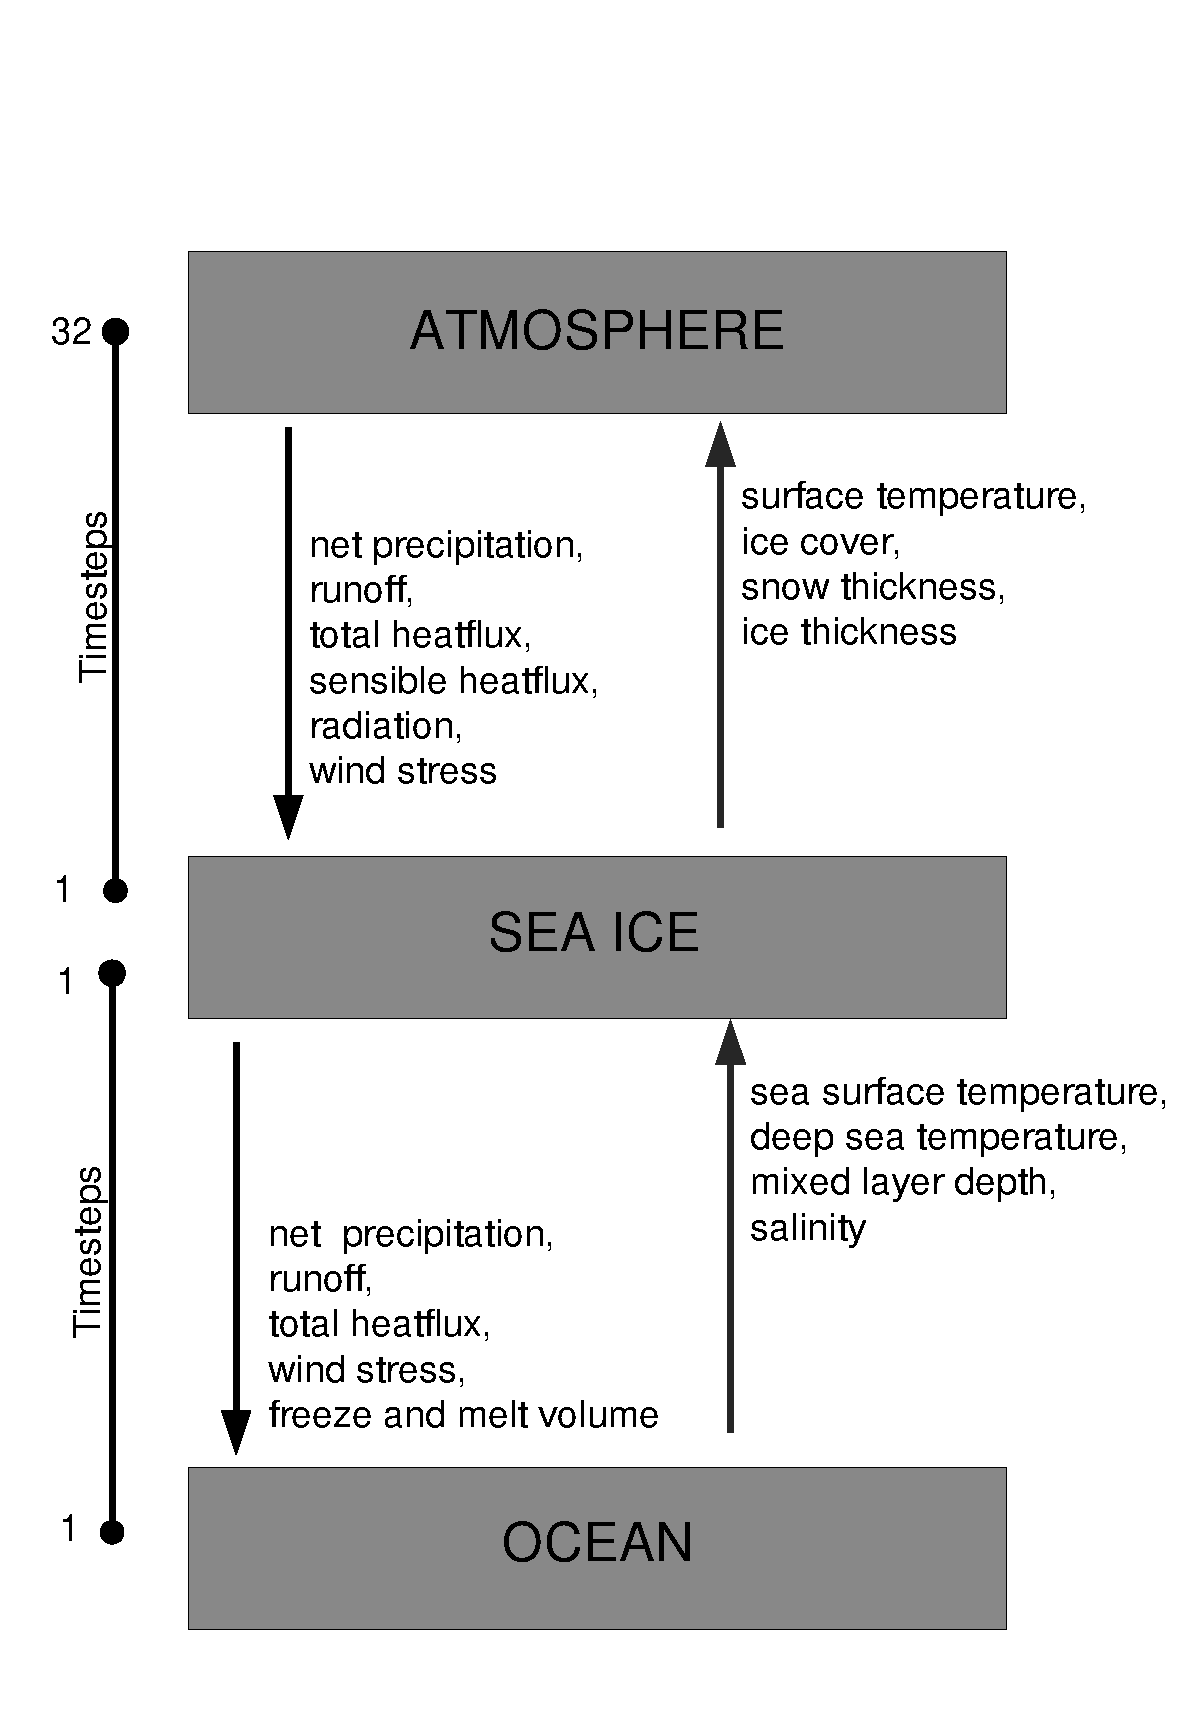
\includegraphics[width={14cm}]{Pics/modules_icemod_couple}
\caption[]{Schematic illustration of the model coupling.}
\label{couplefig}
\end{figure}

\begin{figure}[p]
\vspace{-2cm}
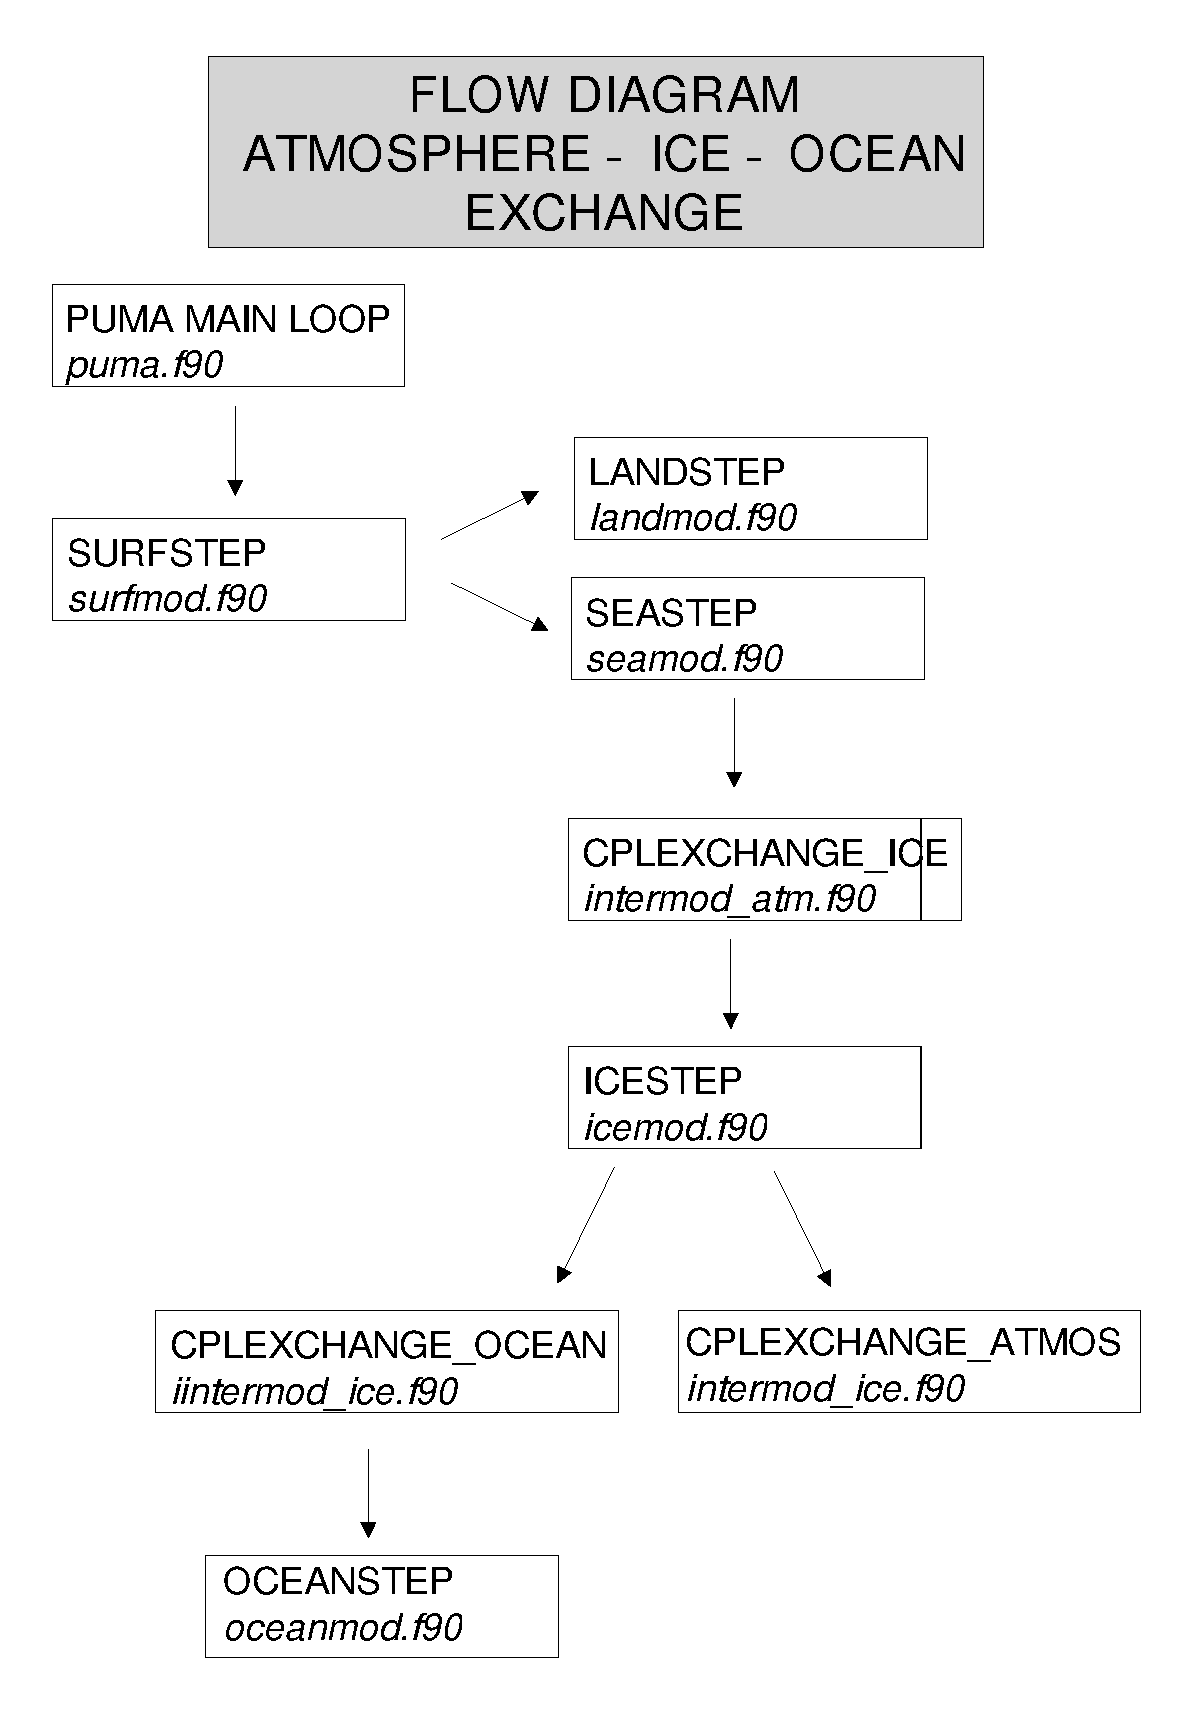
\includegraphics[width={14cm}]{Pics/modules_icemod_pumaflow}
\caption[]{Subroutine flow when no external coupler is used.}
\label{pumaflowfig}
\end{figure}


%----------------------------------------------------------------------------

\clearpage
\begin{center}
\begin{tabular}{|p{14cm}|}
\hline
\vspace{-5mm} \section{icemod.f90} \vspace{-5mm} \\
\hline
\vspace{1mm} {\bf General} The module {\module icemod.f90}
contains subroutines to compute sea ice cover and thickness.
The interface to the main PLASIM module is given by the subroutine
{\sub icestep}, which is called by {\sub cplexchange\verb#_#ice}
(defined in {\module intermod\verb#_#atm.f90}), which is called by
{\sub seastep} (defined in {\module seamod.f90}). \vspace{3mm} \\
\hline
\vspace{1mm} {\bf Input/Output} {\module icemod.f90} requires the file
{\file ice\verb#_#flxcor} if NFLXCORR is set to a negative value.
If NOUTPUT is set to 1, the output files {\file fort.75} containing
global fields of ice model data and the file {\file fort.76}
containing diagnostic ice data are produced (for details,
see the reference manual). Both output files are in service format.
The module is controlled by the namelist {\nam icepar} in the file
{\file ice\verb#_#namelist}. \vspace{1mm} \\
\begin{tabular}{p{3cm} p{2cm} p{6cm} p{2cm}}
Parameter  & Type    & Purpose 					& default \\
NDIAG	   & INTEGER & Diagnostic output every NDIAG time steps	& 160	  \\
NOUT	   & INTEGER & Model data output every NOUT time steps	& 32	  \\
NOUTPUT	   & INTEGER & Icemodel output (0=no,1=yes)		& 1	  \\
NFLXCORR   & INTEGER & Time constant for restoring $(>0)$, no flux correction $(=0)$, use fluxcorrection from file $(<0)$ & $360\,d$ \\
\end{tabular} \vspace{3mm} \\
\hline
\vspace{2mm} {\bf Structure} {\module icemod.f90} uses the module
{\modu icemod} which is not dependent on the module {\modu pumamod}.
Subroutine {\sub iceini} reads the namelist and, when required,
the flux correction from the file {\file ice\verb#_#flxcor}.
Subroutine {\sub icestep} calls {\sub cplexchange\verb#_#atmos}
(defined in {\module intermod\verb#_#ice}) to get the atmospheric
forcing fields. If the {\nam sea\verb#_#namelist} parameter NICE is
set to 1, the subroutine {\sub subice} is called, which calculates
ice cover and thickness. Otherwise, climatological data, interpolated
to the current time step by {\sub iceget} are used. If an ice cover
is present, the surface temperature is calculated in {\sub skintemp}.
Otherwise, the surface temperature is set to the sea surface temperature
calculated by the ocean model. Every NCPL\verb#_#ICE\verb#_#OCEAN
(defined in {\nam sea\verb#_#namelist}) time steps, the external
subroutine {\sub cplexchange\verb#_#ocean} (defined in
{\module intermod\verb#_#ice}) is called to pass the atmospheric
forcing to and retrieve oceanic data from the ocean module
{\module oceanmod.f90}. The oceanic data is used for ice calculations
in the next time step. \vspace{3mm} \\
\hline
\end{tabular}
\end{center} 

%--------------------------------------------------------------------------------

\clearpage
\begin{center}
\begin{tabular}{|p{14cm}|}
\hline
\vspace{-5mm} \section{oceanmod.f90} \vspace{-5mm} \\
\hline
\vspace{1mm} {\bf General} The module {\module oceanmod.f90} contains
a mixed layer ocean model, i.e. subroutines to compute sea surface
temperature and mixed layer depth. The interface to the main PLASIM
module is via the module {\module icemod.f90} given by the subroutine
{\sub oceanstep}, which is called by {\sub cplexchange\verb#_#ocean}
(defined in {\module intermod\verb#_#ice}).  \vspace{3mm} \\
\hline
\vspace{1mm} {\bf Input/Output} {\module oceanmod.f90} requires the file {\file ocean\verb#_#flxcor} if NFLXCORRSST or NFLXCORRMLD is set to a negative value. If NOUTPUT is set to 1, the output file {\file fort.31} containing global fields of ocean model data in service format is produced (for details, see the ice modul section of the reference guide). The module is controlled by the namelist {\nam oceanpar} in the file {\file ocean\verb#_#namelist}. \vspace{1mm} \\
\begin{tabular}{p{3cm} p{2cm} p{6cm} p{2cm}}
Parameter   & Type    & Purpose 			        & default \\
NDIAG	    & INTEGER & Diagnostic output every NDIAG time steps	& 480	  \\
NOUT	    & INTEGER & Model data output every NOUT time steps	& 32	  \\
NOUTPUT	    & INTEGER & Oceanmodel output (0=no,1=yes)		& 1	  \\
NFLXCORRMLD & INTEGER & Time constant for restoring mixed layer depth $(>0)$, no flux correction $(=0)$, use fluxcorrection from file $(<0)$ & $60\,d$ \\
NFLXCORRSST & INTEGER & Time constant for restoring sea surface temperature $(>0)$, no flux correction $(=0)$, use fluxcorrection from file $(<0)$ & $60\,d$ \\
\end{tabular} \vspace{3mm} \\
\hline
\vspace{2mm} {\bf Structure} {\module oceanmod.f90} uses the module
{\modu oceanmod} which is not dependent on the module {\modu pumamod}.
Subroutine {\sub oceanini} reads the namelist and, when required,
the flux corrections from the file {\file ocean\verb#_#flxcor}.
Subroutine {\sub oceanstep} calls {\sub mixocean}, which calculates
mixed layer depth and temperature. If an ice cover is present, mixed
layer depth is set to the climatological value and the sea surface
temperature is set to the freezing temperature. For details of the
mixed layer model, see the Planet Simulator Reference Manual.  \vspace{3mm} \\
\hline
\end{tabular}
\end{center} 

%------------------------------------------------------------------------




\chapter{Parallel Program Execution}
\section{Concept}

The {\bf Planet Simulator} is coded for parallel execution
on computers with multiple CPU's or networked machines.
The implementation uses MPI (Message Passage Interface),
that is available for nearly every operating system
{\url{http://www.mcs.anl.gov/mpi}}.

In order to avoid maintaining two sets of source code
for the parallel and the single CPU version, all
calls to the MPI routines are encapsulated into a module.
Users, that want to compile and execute the parallel
version use the module
{\bf mpimod.f90} and the commands {\bf mpif90}
for compiling and {\bf mpirun} for running.

If MPI is not implemented or the single CPU
version is sufficient, {\bf mpimod\_stub.f90}
is used instead of {\bf mpimod.f90}.
Also remove or comment the line:
\begin{verbatim}
!     use mpi
\end{verbatim}
and set the number of processors to 1:
\begin{verbatim}
      parameter(NPRO = 1)
\end{verbatim}




\section{Parallelization in Gridpoint Domain}

The data arrays in gridpoint domain are either 
three-dimensional e.g. gt(NLON, NLAT, NLEV) referring
to an array organized after longitudes, latitudes and levels,
or two-dimensional, e.g. gp(NLON, NLAT).
The code is organized such, that there are no dependencies
in latitudinal direction, while in gridpoint domain.
Such dependencies are resolved during the Legendre-Transformations.
So the the partitioning of the data is done in latitudes.
The program can use as many CPU's as latitudes with the extreme
of every CPU doing the computations for a single latitude.
There is the restriction however, that the number of latitudes
(NLAT) divided by the number of processors (NPRO), giving
the number of latitudes per process (NLPP) must have zero
remainder. E.g. A T31 resolution uses $NLAT=48$.
Possible values for NPRO are then 1, 2, 3, 4, 6, 8, 12, 16, 24, and 48.

All loops dealing with a latitudinal index look like:
\begin{verbatim}
      do jlat = 1 , NLPP
         ....
      enddo
\end{verbatim}

There are, however, many subroutines, with the most prominent
called {\bf calcgp}, that can fuse latitudinal and longitudinal
indices. In all these cases the dimension NHOR is used.
NHOR is defined as: $NHOR = NLON * NLPP$ in the 
pumamod - module. The typical gridpoint loop that looks like:

\begin{verbatim}
      do jlat = 1 , NLPP
         do jlon = 1 , NLON
            gp(jlon,jlat) = ...
         enddo
      enddo
\end{verbatim}

is then replaced by the faster executing loop:

\begin{verbatim}
      do jhor = 1 , NHOR
         gp(jhor) = ...
      enddo
\end{verbatim}

\section{Parallelization in Spectral Domain}

The number of coefficients in spectral domain (NRSP)
is divided by the number of processes (NPRO) giving
the number of coefficients per process (NSPP).
The number is rounded up to the next integer and the
last process may get some additional dummy elements,
if there is a remainder in the division operation.

All loops in spectral domain are organized like:

\begin{verbatim}
      do jsp = 1 , NSPP
         sp(jsp) = ...
      enddo
\end{verbatim}

\section{Synchronization points}

All processes must communicate and have therefore to
be synchronized at following events:

\begin{itemize}

\item Legendre-Transformation: 
This involves changing from latitudinal partitioning to
spectral partitioning and such some gather and scatter
operations.

\item Inverse Legendre-Transformation:
The partitioning changes from spectral to latitudinal
by using gather, broadcast, and scatter operations.

\item Input-Output:
All read and write operations must be done only by
the root process, who gathers and broadcasts or
scatters the information as desired.
Code that is to be executed by the root process exclusively is 
written like:

\begin{verbatim}
   if (mypid == NROOT) then
      ...
   endif
\end{verbatim}

NROOT is typically 0 in MPI implementations,
mypid (My process identification) is assigned by MPI.

\end{itemize}


\section{Source code}

It needs some discipline in order to maintain parallel code.
Here are the most important rules for changing or adding code
to the {\bf Planet Simulator}:

\begin{itemize}

\item Adding namelist parameters:
   All namelist parameters must be broadcasted after reading
   the namelist. (Subroutines mpbci, mpbcr, mpbcin, mpbcrn)

\item Adding scalar variables and arrays:
   Global variables must be defined in a module header
   and initialized. 

\item Initialization code:
   Initialization code, that contains dependencies on
   latitude or spectral modes must be done by the
   root process only and then scattered from there
   to all child processes.

\item Array dimensions and loop limits:
   Always use parameter constants (NHOR, NLAT, NLEV, etc.)
   as defined in
   pumamod.f90 for array dimensions
   and loop limits. 

\item Testing:
   After significant code changes the program should be tested 
   in single and in multi-CPU configuration. The results
   of a single CPU run is usually not exactly the same as the
   result of a multi-CPU run due to effects in
   rounding. But the results should show only small
   differences during the first timesteps.

\item Synchronization points:
   The code is optimzed for parallel execution and minimizes
   therefore communication overhead. The necessary communication
   code is grouped around the Legendre-transformations.
   If more scatter/gather operations or other communication
   routines are to be added, they should be placed
   just before or after the execution of the calls to the
   Legendre-Transformation. Any other place would degrade
   the overall performance in introducing additional
   process synchronization.

\end{itemize}




\chapter{Graphical User Interface}
\label{chap_GUI}
\section{Graphical user interface (GUI)}

\begin{figure}
   \centering
   \includegraphics[width=14cm]{Pics/mostsnap}
   \caption[]{Screenshot of Model Starter (MoSt)}
   \label{mostsnap}
\end{figure}

{\bf PUMA} may be used in the traditional fashion,
with shell scripts, batch jobs, and network queuing 
systems. This is useful for long running simulations
on complex machines and number crunchers, such as vector 
computers, massive parallel computers and workstation clusters.
However, there is now a more convenient method.
A graphical user interface (GUI) has been provided, which 
can be used for parameter configuration during model setup, and 
for interaction between the user and the model.


PUMA is setup and configured using the first
GUI module named {\module MoSt} ({\bf Mo}del {\bf St}arter, 
screenshot in \ref{mostsnap}). 
{\module MoSt} is the fastest way to get the
model running. It gives access to the most important parameters of
the model which are preset to the frequently used values.
The model can be started with a mouse click on the button
labelled ``Save \& Run'' either with the standard parameter setting,
or after editing the parameters in the MoSt window.
Some parameters, like horizontal and vertical resolution
or the number of processors, require that a new executable is built
(compile, link and load). MoSt achieves
this by generating and executing build scripts,
that perform the necessary code changes and
create the required executables.
Other parameters defining startup and
boundary conditions or other settings, can
be edited with MoSt. After they have been checked for
correct range and for consistency with other parameters, they
are written to the model's namelist file.

Using these settings
MoSt generates a run script for the simulation.
The user then has the choice of leaving MoSt and
starting the simulation under the control of the GUI
immediately, or of leaving MoSt with the scripts ready
to run. This second alternative is useful for users who
want to include setup modifications beyond the scope of MoSt,
or who want to run the model without the GUI.

There is also a simple graphical editor for the topography.
Check the box Orography and then use the mouse to mark
elliptic areas in the topographic display.
Enter a value for raising (positive) or lowering (negative) the area
and press the button labelled {\bf Preprocess}.
The preprocessor will be built and executed, and a new
topography will be computed and written to the start file.

Another editor is the Mode Editor for spherical harmonics.
Green modes are enabled, red modes are disabled.
This feature can be used to specify runs with only certain
modes of spherical harmonics being active.
LMB, MMB and RMB refer to the left, middle, and right mouse
buttons respectively. You may toggle individual modes (press LMB)
or whole lines (press RMB) and columns (press MMB). 
Currently the Mode Editor can only be used
for PUMA in the T21 resolution.

\begin{figure}
   \centering
   \includegraphics[width=14cm]{Pics/guisnap}
   \caption[]{Screenshot of Graphical User Interface (GUI)}
   \label{guisnap}
\end{figure}

The GUI for running PUMA
(Figure \ref{guisnap})
has two main uses. The first is to display the
model arrays in suitable representations.
Current implementations are:
\begin{itemize}
\item{Zonal mean cross sections}
\item{Horizontal global fields in cylinder or polar projection}
\item{Horizontal particle tracer in cylinder or polar projection}
\item{Longitude-time (Hovmoeller) diagrams}
\item{Longitude-level diagrams}
\item{Amplitudes of spherical harmonic coefficients}
\item{Time series}
\item{Numerical values}
\end{itemize}

In the case of horizontal global grids, pressing the MMB 
toggles between cylinder and polar projection. If the grid is
a single level of a three dimensional field like u or v,
the level being shown can be decreased with the LMB or increased with the RMB.
For Hovmoeller and longitude height sections the LMB and RMB can
be used to select the latitude.

The second use of the GUI is to allow the user to change
selected model variables during the model run.
It is not necessary, though possible, to pause the
model while changing variables. Changes to model variables
are written to the output file after being checked
by the GUI for the appropriate range of values and the 
maximum possible change per timestep, because 
a rapid parameter change or a choice of values beyond the normal
range may cause the model to crash.

All model variables, which are candidates for display
or for interactive changes, have special code to communicate
with PUMA. The experienced modeller
can add new code for additional variables using the existing
communication code as a template. Thus all model fields
or even fields received via coupling with other models
can be shown on the GUI display.

Both, MoSt and the GUI are implemented using Xlib (X11R5),
which is a library of routines for graphics and event communication.
As this library is part of every UNIX/Linux operating system
and is the base of all desktop environments, there is no need
to install additional software for running MoSt and the GUI.
Another important  property of Xlib is full network transparency.
The display of MoSt and the GUI is not confined to the machines
running the programs or the model. In fact, the best
performance is obtained by running the PUMA on
two or four CPUs of remote servers while displaying
the GUI on the user's workstation.
In summary, MoSt and the GUI programs automate many tedious tasks,
minimize the time to become familiar with the PUMA,
and make debugging and parameter tuning much easier.
More types of presentation, coordinate projections
and interactivity are being developed.
A graphical preprocessor with editor for boundary
conditions and a graphical postprocessor are part of the planned
future expansion
to build an almost complete environment for modellers.

\section{GUI configuration}

On initialization, the GUI reads its configuration from a file called
{\bf GUI.cfg} which must be present in the current directory.
MoSt copies the file {\bf GUI.cfg} from the ../dat/ directory
to the run directory while building PUMA.
After reading {\bf GUI.cfg} an attempt is made to read the file
{\bf GUI\_last\_used.cfg}. This file is always written at the end
of a GUI controlled simulation. So one may rearrange and position
GUI windows during a run and the new layout will be saved to the
file {\bf GUI\_last\_used.cfg}. In order to make this user
layout the default for te following runs, just copy this file:
\begin{verbatim}
Most15/puma/run$ cp ../dat/GUI.cfg ../dat/GUI.cfg.old
Most15/puma/run$ cp GUI_last_used.cfg ../dat/GUI.cfg
\end{verbatim}
MoSt will then copy your new layout to the run directory at 
the next invocation.

The {\bf GUI.cfg} is a text file that may also be edited manually.
There is a section for each window (counting from 0 to 8) which
looks like:

\begin{verbatim}
[Window 00]                       <- window number (0..8)
Array:CSU                         <- array name
Plot:ISOCS                        <- picture type
Palette:U                         <- colour palette
Title:Zonal Wind [m/s]            <- window title
Geometry:  529  299    2    3     <- width height left top

[Window 01]
Array:SPAN
Plot:ISOSH
Palette:AMPLI
Title:Spherical Harmonics Ps
Geometry:  529  299  535    3

...

\end{verbatim}

Possible values for these items are:

\subsection{Array}
\begin{tabular}{|l|l|}
\hline
Name     & Description \\
\hline
CSU      & Cross Section U - Zonal mean zonal wind \\
CSV      & Cross Section V - Zonal mean meridional wind \\
CST      & Cross Section T - Zonal mean temperature \\
SPAN     & Spherical harmonic coefficients of surface pressure \\
GU       & Three dimensional grid of zonal wind \\
GV       & Three dimensional grid of meridional wind \\
GP       & Grid of surface pressure \\
SCALAR   & Selected scalars for time series and tables \\
\hline
\end{tabular}

\subsection{Plot}
\begin{tabular}{|l|l|}
\hline
Name     & Description \\
\hline
   ISOHOR & Isolines and colouring of horizontal grids \\
   ISOCS &  Isolines and colouring of cross sections \\
   ISOHOV & Colouring of Hovmoeller diagram \\
   ISOTS &  Timeseries \\
   ISOTAB & Tables \\
   ISOSH &  Coloured amplitudes \\
   ISOLON & Isolines and colouring of longitude height section \\
   ISOTRA & Show the horizontal wind components with moving particles \\
\hline
\end{tabular}

\subsection{Palette}
\begin{tabular}{|l|l|l|}
\hline
Name     & Range & Description  \\
\hline
   AUTO & automatic & rainbow colours \\
   U &    -10 .. 50 & rainbow colours \\
   V &    -10 .. 10 & rainbow colours \\
   T &    -50 .. 50 & blue - red \\
   P &    985 .. 1025 & blue - red \\ 
   Q &      0 .. 60 & rainbow colours \\
   MARST & -90 .. 0 & blue -red \\
   AMPLI & 0 .. 12 & blue - green -red \\
   VEG   & 0 .. 100 & shades of green \\
\hline
\end{tabular}

\subsection{Title}
The title item may contain any text, but keep it short.
The length of the window's title bar is limited.
The words {\em Latitude} and {\em Level} have special
features in conjunction with three-dimensional arrays,
where the user may scroll the level or latitude.
The GUI will insert the level number after the word 
{\em Level} or the latitude after the word {\em Latitude}.

\subsection{Geometry}
The four integers following the geometry item describe
the size and screen position of the window.
The first two parameters refer to width and height in 
screen pixels. These are the sizes of the inner window.
The title bar, the border and any other decorations are not counted.
The third and fourth parameter set the x and y coordinates of the
upper left corner of the window, again without borders.
If the geometry item is not defined, the GUI will
initialize the window's geometry depending on the screen size.




\chapter{Postprocessor Pumaburner}
\label{Pumaburner}
\section{Introduction}

The {\bf Pumaburner} is a postprocessor for the {\bf Planet Simulator}
and the {\bf PUMA} model family.
It's the only interface between {\it raw} model data output
and diagnostics, graphics, and user software.

The output data of the {\bf Planet Simulator} are stored as
packed binary (16 bit) values using the model representation.
Prognostic variables like temperature, divergence, vorticity,
pressure, and humidity are stored as coefficients of spherical harmonics
on $\sigma$ levels. Variables like radiation,
precipitation, evaporation, clouds, and other fields of the
parameterization package are stored on Gaussian grids.

The tasks of the {\bf Pumaburner} are:
\begin{itemize}
\item Unpack the {\it raw} data to full real representation.
\item Transform variables from the model's representation
      to a user selectable format, e.g. grids,
      zonal mean cross sections, fourier coefficients.
\item Calculate diagnostic variables, like vertical velocity,
      geopotential height, wind components, etc.
\item Transfrom variables from $\sigma$ levels to user
      selectable pressure levels.
\item Compute monthly means and standard deviations.
\item Write selected data either in SERVICE, GRIB, or NetCDF format
      for further processing.
\end{itemize}

\section{Usage}

\begin{verbatim}
pumaburn4 [options] InputFile OutputFile <namelist >printout
     option -h : help (this output)
     option -c : print available codes and names
     option -d : debug mode (verbose output)
     option -g : Grib   output (override namelist option)
     option -n : NetCDF output (override namelist option)
     option -m : Mean=1 output (override namelist option)
     InputFile : Planet Simulator or PUMA data file
    OutputFile : GRIB, SERVICE, or NetCDF format file
      namelist : redirected <stdin>
      printout : redirected <stdout>
\end{verbatim}

\section{Namelist}

The namelist values control the selection, coordinate system
and output format of the postprocessed variables.
Names and values are not case sensitive.
You can assign values to the following names: \vspace{0.4cm}

\begin{tabular}{|l|c|l|l|l|}
\hline
Name   & Def. & Type & Description & Example \\
\hline
{\bf HTYPE  }& S & char & Horizontal type               & HTYPE=G \\
{\bf VTYPE  }& S & char & Vertical type                 & VTYPE=P \\
{\bf MODLEV }& 0 & int  & Model levels                  & MODLEV=2,3,4 \\
{\bf hPa    }& 0 & real & Pressure levels               & hPa=500,1000 \\
{\bf CODE   }& 0 & int  & ECMWF field code              & CODE=130,152 \\
{\bf GRIB   }& 0 & int  & GRIB output selector          & GRIB=1 \\
{\bf NETCDF }& 0 & int  & NetCDF output selector        & NETCDF=1 \\
{\bf MEAN   }& 1 & int  & Compute monthly means         & MEAN=0 \\
{\bf HHMM   }& 1 & int  & Time format in Service format & HHMM=0 \\
{\bf HEAD7  }& 0 & int  & User parameter                & HEAD7=0815 \\
{\bf MARS   }& 0 & int  & Use constants for planet Mars & MARS=1 \\
{\bf MULTI  }& 0 & int  & Process multiple input files  & MULTI=12 \\
\hline
\end{tabular}

\section{HTYPE}

{\bf HTYPE} accepts the first character of the following string.
Following settings are equivalent: HTYPE = S, HTYPE=Spherical Harmonics
HTYPE = Something. Blanks and the equal-sign are optional. \\
Possible Values are:

\begin{tabular}{|l|l|l|}
\hline
   Setting   & Description          & Dimension for T21 resolution   \\
\hline
   HTYPE = S & Spherical Harmonics  & (506):(22 * 23 coefficients)   \\
   HTYPE = F & Fourier Coefficients & (32,42):(latitudes,wavenumber) \\
   HTYPE = Z & Zonal Means          & (32,levels):(latitudes,levels) \\
   HTYPE = G & Gauss Grid           & (64,32):(longitudes,latitudes) \\
\hline
\end{tabular}

\section{VTYPE}

{\bf VTYPE} accepts the first character of the following string.
Following settings are equivalent: VTYPE = S, VTYPE=Sigma
VTYPE = Super. Blanks and the equal-sign are optional. \\
Possible Values are:

\begin{tabular}{|l|l|l|}
\hline
   Setting   & Description          & Remark \\
\hline
   VTYPE = S & Sigma (model) levels & Some derived variables are not available \\
   VTYPE = P & Pressure levels      & Interpolation to pressure levels \\
\hline
\end{tabular}

\section{MODLEV}

{\bf MODLEV} is used in combination with {\bf VTYPE = S}.
If VTYPE is not set to Sigma, the contents of MODLEV are ignored.
MODLEV is an integer array that can get as many values as there are
levels in the model output. The levels are numbered from top of
the atmosphere to the bottom. The number of levels and the 
corresponding sigma values are listed in the pumaburner printout.
The outputfile orders the level according to the MODLEV values.
MODLEV=1,2,3,4,5 produces an output file of five model levels
sorted from top to bottom, while MODLEV=5,4,3,2,1 sorts them
from bottom to top.

\section{hPa}

{\bf hPa} is used in combination with {\bf VTYPE = P}.
If VTYPE is not set to Pressure, the contents of hPa are ignored.
hPa is a real array that accepts pressure values with the
units hectoPascal or millibar. All output variables will be
interpolated to the selected pressure levels.
There is no extrapolation on the top of the atmosphere.
For pressure values, that are lower than that of the model's
top level, the top level value of the variable is taken.
The variables temperature and geopotential height are extrapolated
if the selected pressure is higher than the surface pressure.
All other variables are set to the value of the lowest mode level
for this case. The outputfile contains the levels in the same order
as set in hPa. Example: hpa = 100,300,500,700,850,900,1000.

\section{MEAN}

{\bf MEAN} can be used to compute montly means and/or deviations.
The Pumaburner reads date and time information from the model file
and handles different lengths of months and output intervals correctly.

\begin{tabular}{|l|p{12cm}|}
\hline
Setting & Description \\
\hline
        MEAN  =  0 & Do no averaging - all terms are processed. \\

        MEAN  =  1 & Compute and write monthly mean fields.
                     Not for spherical harmonics, Fourier coefficients or
                     zonal means on sigma levels. \\

        MEAN  =  2 & Compute and write monthly deviations.
                     Not for spherical harmonics, Fourier coefficients or
                     zonal means on sigma levels.
                     Deviations are not available for NetCDF output. \\

        MEAN  =  3 & Combination of MEAN=1 and MEAN=2.
                     Each mean field is followed by a deviation
                     field with an identical header record.
                     Not for spherical harmonics, Fourier coefficients or
                     zonal means on sigma levels. \\
\hline
\end{tabular}

\section{Format of output data}

The {\bf pumaburner} supports three different output formats:

\begin{itemize}
\item {\bf GRIB} (GRIdded Binary) WMO standard for gridded data.
\item {\bf NetCDF} (Network Common Data Format)
\item {\bf Service} Format for user readable data (see below).
\end{itemize}

For more detailed descriptions see for example:

{\url{http://www.nws.noaa.gov/om/ord/iob/NOAAPORT/resources/}}

\begin{tabular}{|l|l|p{10cm}|}
\hline
Setting & Description \\
\hline
   GRIB = 1 & NetCDF = 0 & The output file is written GRIB format.
                     This option can be used only for
                     HTYPE=Spherical Harmonics or HTYPE=Gauss Grid. \\
   GRIB = 0 & NetCDF = 1 & The output file is written in NetCDF format.
                     This option can be used for HTYPE=Gauss Grid only. \\
   GRIB = 0 & NetCDF = 0 & The output file is written in Service format.
                     This is the preferred format for user programs.
                     For a detailed description see the following section. \\
   GRIB = 1 & NetCDF = 1 & Illegal combination. \\
\hline
\end{tabular}

\section{SERVICE format}

     The SERVICE format uses the following structure:
     The whole file consists of pairs of
     header records and data records.
     The header record is an integer array of 8 elements.

\begin{verbatim}
     head(1) = ECMWF field code
     head(2) = modellevel or pressure in [Pa]
     head(3) = date  [yymmdd]  (yymm00 for monthly means)
     head(4) = time  [hhmm]  or [hh] for HHMM=0
     head(5) = 1. dimension of data array
     head(6) = 2. dimension of data array
     head(7) = may be set with the parameter HEAD7
     head(8) = experiment number (extracted from filename)

     Example for reading the SERVICE format (GRIB=0 , NETCDF=0)

     INTEGER HEAD(8)
     REAL    FIELD(64,32)     ! dimensions for T21 grids
     READ (10,ERR=888,END=999) HEAD
     READ (10,ERR=888,END=999) FIELD
     ....
 888 STOP 'I/O ERR'
 999 STOP 'EOF'
     ....
\end{verbatim}

\section{HHMM}

\begin{tabular}{|l|p{12cm}|}
\hline
Setting & Description \\
\hline
  HHMM  =  0 & head(4) shows the time in hours (HH). \\
  HHMM  =  1 & head(4) shows the time in hours and minutes (HHMM). \\
\hline
\end{tabular}

\section{HEAD7}
The 7th. element of the header is reserved for the user.
It may be used for experiment numbers, flags or anything else.
Setting HEAD7 to a number exports this number to every header record
in the output file (SERVICE format only).

\section{MARS}
This parameter is used for processing simulations of the Mars atmosphere.
Setting MARS=1 switches gravity, gas constant and planet radius
to the correct values for the planet Mars.

\section{MULTI}
The parameter MULTI can bes used to process a series of input data
within one run of the pumaburner. Setting MULTI to a number (n)
tells the pumaburner to procees (n) input files.
The input files must follow one of the following two rules:
\begin{itemize}
\item YYMM rule: The last four characters of the filename 
                 contain the data in the form YYMM.
\item .NNN rule: The last four characters of the filename
                 consist of a dot followed ny a 3-digit sequence number.
\end{itemize}

\begin{verbatim}
Examples:

Namelist contains MULTI=3
Command: pumaburn <namelist >printout run.005 out
pumaburn processes the files <run.005> <run.006> <run.007>

Namelist contains MULTI=4
Command: pumaburn <namelist >printout exp0211 out
pumaburn processes the files <exp0211> <exp0212> <exp0301> <exp0302>
\end{verbatim}

\section{Namelist example}
\begin{verbatim}
       VTYPE  = Pressure
       HTYPE  = Grid
       CODE   = 130,131,132
       hPa    = 200,500,700,850,1000
       MEAN   = 0
       GRIB   = 0
       NETCDF = 0
\end{verbatim}

    This namelist will write Temperature(130), u(130) and v(131)
    on pressure levels 200hPa, 500hPa, 700hPa, 850hPa and 1000hPa.
    The output interval is the same as found on the model data,
    e.g. every 12 or every 6 hours (MEAN=0). The output format
    is SERVICE format.

\section{Troubleshooting}
If the pumaburner reports an error or doesn't produce 
the expected results, try the following:

\begin{itemize}

\item Check your namelist, especially for invalid codes, types and levels.

\item Run the pumaburner in debug-mode by using the option -d.
Example:
\begin{verbatim}
pumaburn <namelist >printout -d data.in data.out
\end{verbatim}

This will print out some details like parameters and memory allocation
during the run. The additional information may help to detect
the problem.

\item Not all combinations of HTYPE, VTYPE, and CODE are valid.
Try to use HTYPE=Grid and VTYPE=Pressure before switching to
exotic parameter combinations.

\end{itemize}



\chapter{Graphics}
\section{Grads}
In this section, visualisation using the graphics package \verb#GrADS#
({\bf Gr}id {\bf A}nalysis and {\bf D}isplay {\bf S}ystem) is
described. A useful Internet site for reference and for installation
instructions is
\begin{quote}
{\url{http://grads.iges.org/grads/grads.html}}.
\end{quote}
The latest version of \verb#GrADS# can handle data in \verb#NetCDF#
format via the command \verb#sdfopen#.
Any file produced by the \verb#Pumaburner# with the option NETCDF=1
can be read directly by \verb#GrADS#.
For files in the \verb#SERVICE# format is possible to use
a converter, which translates from the \verb#SERVICE# format into \verb#NetCDF#.
But in the following it is assumed that the \verb/PUMA/ output has been
postprocessed into the \verb#SERVICE# format with the \verb#Pumaburner# and that the
resulting file is called \verb/puma.srv/. Using the option -g for the \verb#Pumaburner# 
creates the related GrADS control file \verb/puma.ctl/.
Monthly mean data is either obtained
directly from the \verb#Pumaburner# (\verb#namelist# parameter
\verb#MEAN=1#, see section \ref{Pumaburner}) or via a
\verb/CDO/ command:
\begin{quote}
\verb/cdo monmean puma.srv puma_m.srv/
\end{quote}
\noindent Information on the {\bf C}limate {\bf D}ata {\bf O}perators ({\bf CDO}'s)
can be found in the \verb#CDO User's Guide# at
\begin{quote}
 {\url{http://www.mpimet.mpg.de/fileadmin/software/cdo/}}.
\end{quote}
When the \verb#GrADS# control file was not created via the \verb#Pumaburner# 
option -g, it can be done by the command:

\begin{quote}
\verb#srvctl puma_m.srv#
\end{quote}
\noindent which creates the file \verb/puma_m.ctl/. 
It contains information on the grid, time steps, and variable names. The file
\verb/puma_m.srv/ is still needed in addition.
The program
\verb#srvctl.f90# is one of the post-processing tools available at
\begin{quote}
{\url{http://mi.uni-hamburg.de/puma/}}.
\end{quote}
If you chose to compile it yourself, please read the comments in the
first few lines of the program text. Sometimes the
\verb/srvctl/ tool has difficulty calculating an appropriate time axis 
from the data headers of the data records, so you should check this. 
In particular the number of days per year is concerned: \verb#GrADS# may assume 365
days per year even though the data header says 360 days per year.
This is an example of what the \verb/puma_m.ctl/ should look like:
\begin{verbatim}
DSET ^puma_m.gra
UNDEF 9e+09
XDEF     64 LINEAR   0.0000   5.6250
OPTIONS YREV
YDEF     32 LEVELS 
  -85.7606  -80.2688  -74.7445  -69.2130  -63.6786  -58.1430  -52.6065  -47.0696
  -41.5325  -35.9951  -30.4576  -24.9199  -19.3822  -13.8445   -8.3067   -2.7689
    2.7689    8.3067   13.8445   19.3822   24.9199   30.4576   35.9951   41.5325
   47.0696   52.6065   58.1430   63.6786   69.2130   74.7445   80.2688   85.7606
ZDEF      5 LEVELS 
     20000
     50000
     70000
     85000
    100000
TDEF 12 LINEAR 00:00Z01jan0001        1mo
VARS  3
c130     5 99    130     0     0
c131     5 99    131     0     0
c132     5 99    132     0     0
ENDVARS
\end{verbatim}
Here, since we are handling monthly mean data, the line starting 
with \verb/TDEF/ ends with \verb/1mo/. When the \verb/PUMA/ output is used
without averaging, this should correspond to the output interval given
by the \verb#nwpd# variable used in the \verb#namelist# of your \verb#PUMA#
run (see Appendix \ref{Namelist}). The number of variables
depends on how the Pumaburner was
called. In this example, only three variables were processed, i.e.\ the
temperature (\verb/c130/), the zonal wind (\verb/c131/) and the meridional 
wind (\verb/c132/). Refer to Appendix \ref{Pumacodes} for a list of the codes.
\\
The GrADS program is started by typing \verb/grads/ in a terminal window. 
Then, the data is displayed either by typing commands line-by-line, 
or preferably by using scripts. The following script, called \verb/tglob.gs/, 
displays the monthly mean temperature at 500hPa:
\begin{verbatim}
# tglob.gs
function pass(m)
'reinit'
'open puma_m'
'enable print print.mf'
'set t 'm
'set lev 50000'
'c'
'set gxout shaded'
'd (c130-273.16)'
'cbar.gs'
'set gxout contour'
'd (c130-273.16)'
'draw title Temperature (deg C) 500hPa month 'm
'print'
'disable print'
'!gxps -i print.mf -o tglob'm'.ps'
\end{verbatim}
The variable \verb/m/ at the beginning of the script defines the month 
which should be displayed. It is passed from the terminal with the 
script call. Note that no quotation marks are present in this line, 
since only \verb/GrADS/ specific commands are framed by quotation marks. 
Script commands, variable definitions, if-clauses, etc. are used without 
quotation marks. The script is executed by typing its name, without 
the suffix \verb/.gs/, followed by the number of the month to be shown. 
For example, \verb/tglob 7/ displays the monthly mean temperature at 500hPa
in July. The resulting output file is called \verb/tglob7.ps/. 
\par
\vspace{3mm}
The following script \verb/thh/ displays the time dependent 
temperature (in 1000hPa) of Hamburg. Here, two variables are passed to \verb/GrADS/ to plot, 
the first day and the last day. (Note that here, the file \verb/puma.gra/ 
is opened, which contains data on a daily basis). The call \verb/thh 91 180/ 
displays the temperature in 1000hPa of Hamburg for the spring season 
from April 1st to June 30th.

\begin{verbatim}
# thh.gs
function pass(d1 d2)
'reinit'
'open puma'
'enable print print.mf'
'set lat 53'
'set lon 10'
'set lev 100000'
'set t 'd1' 'd2
'c'
'd (c130-273.16)'
'draw title Temperature (deg C) 1000hPa in Hamburg'
'print'
'disable print'
'!gxps -i print.mf -o thh.ps'
\end{verbatim}

\vspace{3mm}
It is possible to have more than one figure in a plot, which is 
illustrated in the following script. It plots the seasonal means 
of the sea level pressure. The data file is prepared like this:

\begin{verbatim}
cdo selcode,151 puma.srv slp.srv    #code 151 has to be in puma.srv  
cdo seasmean slp.srv slp_sm.srv
srv2gra slp_sm.srv
\end{verbatim}

The command \verb/set vpage/ sets a virtual page inside the graphic 
window. The full window is 11 inch wide and 8.5 inch high, so 
\verb/set vpage 0 5.5 4.25 8.5/ defines the upper left corner. 
If \verb/setlevs=1/ is specified, then the pressure levels as given are used. 
Otherwise, \verb/GrADS/ defines contour levels depending on the data set.

\begin{verbatim}
# slp_sm.gs
setlevs=1
'reinit'
'open slp_sm'
'enable print print.mf'
'c'
'set vpage 0 5.5 4.25 8.5'
'set gxout contour'
if (setlevs=1)
'set clevs 990 995 1000 1005 1010 1015 1020'
endif
'set ccols 1'
'set grads off'
'set t 1'
'd c151/100'
'draw title SLP [hPa] yr 'ny' DJF'
'set vpage 5.5 11 4.25 8.5'
'set gxout contour'
if (setlevs=1)
'set clevs 990 995 1000 1005 1010 1015 1020'
endif
'set ccols 1'
'set grads off'
'set t 2'
'd c151/100'
'draw title yr 'ny' MAM'
'set vpage 0 5.5 0 4.25'
'set gxout contour'
if (setlevs=1)
'set clevs 990 995 1000 1005 1010 1015 1020'
endif
'set ccols 1'
'set grads off'
'set t 3'
'd c151/100'
'draw title yr 'ny' JJA'
'set vpage 5.5 11 0 4.25'
'set gxout contour'
if (setlevs=1)
'set clevs 990 995 1000 1005 1010 1015 1020'
endif
'set ccols 1'
'set grads off'
'set t 4'
'd c151/100'
'draw title yr 'ny' SON'
'print'
'disable print'
'!gxps -c -i print.mf -o slp_sm.ps'
\end{verbatim}

\section{Vis5D}
\begin{quote}
{\it ``Vis5D is a system for interactive visualization of large 5-D
gridded data sets such as those produced by numerical weather
models. One can make isosurfaces, contour line slices, colored slices,
volume renderings, etc of data in a 3-D grid, then rotate and animate
the images in real time. There's also a feature for wind trajectory
tracing, a way to make text annotations for publications, support for
interactive data analysis, etc.''}
\par
\end{quote}
\begin{flushright}
from the Vis5D home page,\\
{\url{http://www.ssec.wisc.edu/~billh/vis5d.html}}
\end{flushright}
\par
\noindent This powerful visualisation tool together with its documentation is
available through the above home page. Vis5D uses its own data format
which makes it necessary to transform your data. Depending on their
format
% (see also section \ref{Filestructure}
 and the flowchart on
{\url{http://puma.dkrz.de/puma/download/map/}} you have the following
choices: If

\begin{itemize}
\item{{\it your data is raw \verb#PUMA# output,}\\
	you need to process it with the \verb#pumaburner#
	postprocessor (see section \ref{Pumaburner}) in order to
	transform it to either
	\verb#NETCDF#} (option \verb#-n# or namelist parameter
	\verb#NETCDF=1#) or \verb#GRIB# (option \verb#-g# or namelist
	parameter \verb#GRIB=1#) and proceed from there.
\item{{\it your data is in \verb#SERVICE# format,}\\
	you need to convert it to either \verb#GRIB#, for
	instance with the \verb#PINGO#s:
\begin{quote}
 \verb#grb copy2 data.srv data_with_grib_metainfo.grb output.grb#,
\end{quote}	
	or \verb#NETCDF#,
	using the program \verb#puma2cdf#, which is available with the
	\verb#PUMA# postprocessing tools. Despite of its name this
	program cannot process raw \verb#PUMA# output but takes
	\verb#SERVICE# format as input. It can as well be called as
	\verb#srv2cdf# which changes its behaviour: oddities of model
	output such as the existence of February, $30^{th}$ are
	then no longer removed.	Once the format is changed proceed from there.}
\item{{\it your data is in \verb#NETCDF# format,}\\
	it can easily transformed to \verb#Vis5D#'s native format by
	means of the program \verb#cdf2v2d#, which is available with
 	the \verb#PUMA# postprocessing tools.}
\item{{\it your data is in \verb#GRIB# format,\\}
	you can find a transformation tool named \verb#Grib2V5d# at\\
	\verb#<http://grib2v5d.sourceforge.net># which offers various
	practical features.}
\end{itemize}
\noindent Once the conversion to \verb#Vis5D#'s native format is
	achieved please follow the instructions from the \verb#Vis5D#
	documentation or, if \verb#Vis5D# is already installed on your
	system, try finding your own way by typing:
\begin{quote}
\verb#vis5d my_data.v5d#
\end{quote}




\chapter{Column Mode and Soundings}
 \section{Setup}

The column mode of the the Planet Simulator is an integral part 
of the full Planet Simulator and not a stand alone model. 
The advantage of this approach is that all options and modules 
available in the full model are automatically included in
the column mode and that no extra maintenance is necessary. 

Technically this is realized by switching off horizontal 
advection and diffusion which leaves us with an independent
column for each grid point. The inclusion of additional options
for boundary conditions allows for runs with synchronized columns.   

Running the Model at the lowest resolution (T1) with  $8$ 
synchronized columns is efficient enough to
run very fast column integrations. Using a standard setup
with $10$ atmospheric layers and a mixed layer ocean one 
can simulate more than $33500$ years per day on a single 
processor PC (3.3 GHZ CPU).

To make full use of the computer power one can setup an ensemble of 
columns by specifying boundary conditions for every grid point 
separately.

\subsection{Basic switches for column setup}

We introduce the macro switch {\bf COLUMN} in the namelist {\it inp}
which is part of the namelist $\mathrm{ \bf puma{\_}namelist}$.
By setting {\bf  COLUMN = 1} a default column mode is initialized by
setting {\bf YMODE = "Column"}, {\bf KICK = 0}, {\bf NADV = 0}
and {\bf NHORDIF = 0}. One can customize the column setup by keeping
the default value {\bf  COLUMN = 0} and by setting the other switches
individually. For more details see the table {\it inp}
in appendix \ref{Namelist}.  

\subsection{Boundary Conditions and forcing}

For the T1 truncation the following lower boundary conditions are specified
by external fields: The land sea mask 
($\mathrm{N002\_surf\_0172.sra}$), 
the surface geopotential ($\mathrm{N002\_surf\_0129.sra}$)
and the surface temperature ($\mathrm{N002\_surf\_0169.sra}$).
The other fields are set by default within the model. Some can be
set by namelist parameters (see description of standard model).

The surface fluxes of heat and moisture in the 
column mode can be influenced by the switch {\bf ZUMIN} 
in the namelist {\it fluxpar} which sets the surface wind 
speed entering the bulk exchange scheme. The default value 
is set to 1 m/s.

Keeping the standard settings the columns will be forced by the solar
forcing corresponding to the grid point where the column is located.
For the T1 truncation this mean that the columns are located approximately
at gaussian latitudes $\pm 35.26^\circ$. The solar forcing corresponds
to the default of the full model. A daily mean insolation is
used with an annual cycle. The solar forcing is also influenced
by the climatological ozon distribution which by default also has
an annual cycle.


\section{Graphical User Interface (GUI)}

To visualize the time evolution of the column model a vertical Hovmoeller 
plot has been added to the GUI (picture type: ISOCOL).
The sounding device can be also used to visualize the vertical profiles at 
an arbitrary grid point of the gaussian grid in the full model. 
By clicking the window the sounding goes from grid point to grid point 
in meridional direction. The longitude can be selected by the switch 
{\bf sellon}, which is a parameter of the {\bf inp} namelist in 
$\mathrm{\bf puma\_namelist}$.  
Using the template $\mathrm{GUI\_sounding.cfg}$ in folder 
{\bf plasim/dat} the GUI is configured for soundings. 
In this case {\bf sellon} can be modified in the control window. 
For more details see chapter \ref{chap_GUI}. 


% \chapter{Diagnostics}
% \section{Fluxes}

% \chapter{Reference Simulation}

\begin{appendix}
\chapter{List of Constants and Symbols}
\newcommand{\e}[1]{\cdot 10^{#1}}
\subsection{List of Constants and Symbols}
\label{locs}
\begin{tabular*}{\textwidth}{l@{\extracolsep\fill}lll}
Symbol         & Definition                       & Value   & Unit \\
\hline \\
$a$       & earth radius                          & $\rm 6371\e{3}$ & $\rm
m$ \\
$A$       & $=D+\vec{V} \cdot \nabla \ln p_s $         &         & $\rm -$ \\
${\cal A}$      &  absorptivity/emissivity                                           &                     & $\rm -$ \\
${\cal A}_S$  & surface emissivity                                              &         &$\rm -$ \\
$B(T)$            & Planck function                    &    &$\rm Wm^{-2}$ \\
$cc$      & cloud cover                 &    & $\rm -$\\
$C_{char}$     & Charnock constant                     & 0.018   & $\rm -$ \\
$C_h$          & transfer coefficient for heat         &         & $\rm -$ \\
$C_m$          & drag coefficient for momentum         &         & $\rm -$ \\
$c_p$          & specific heat of moist air at constant pressure      &         & $\rm J\,
kg^{-1}\, K^{-1}$ \\  
$c_{pd}$  & specific heat of dry air at constant pressure   & 1005.46      & $\rm J\,
kg^{-1}\, K^{-1}$ \\
$c_{pv}$  & specific heat of water vapor at constant pressure    & 1869.46      & $\rm J\,
kg^{-1}\, K^{-1}$ \\
$c_{p_i}$      & specific heat of sea ice              & 2070         & $\rm W\,
s\, kg^{-1}\, K^{-1}$ \\
$c_{p_s}$      & specific heat of snow            & 2090         & $\rm W\,
s\, kg^{-1}\, K^{-1}$ \\
$c_{p_w}$      & specific heat of sea water            & 4180         & $\rm W\,
s\, kg^{-1}\, K^{-1}$ \\
$c_w$          & coefficient for the deep ocean heat flux   & 4       & $\rm W\,
m^{-2}\, K^{-1}$ \\
$C_w$          & wetness factor                   &         & $\rm -$ \\

$D$       & scaled divergence                          &         & $\rm -$ \\

$E$       & evaporation                      &         & $\rm m\,
s^{-1}$ \\
$E_0$          & extrateristical solar flux density         &         & $\rm W\,
m^{-2}$ \\

$f$       & Coriolis parameter $=:2\Omega\sin\varphi$  &         & $\rm
s^{-1}$ \\
$F_p$          & tendency of the first moment$=:\frac{d R_{1}}{d t}$  &    &
$\rm K\, m^2\, s^{-1}$ \\
$F_q$          & tendency of the zeroth moment$=:\frac{d R_{0}}{d t}$ &    &
$\rm K\, m\, s^{-1}$ \\
$F_q$          & surface moisture flux            &         & $\rm kg\,
m^{-2}\, s^{-1}$ \\
$F_T$          & surface sensible heat flux            &         & $\rm W\,
m^{-2}$ \\
$F_u$          & surface zonal wind stress             &         & $\rm Pa$
\\
$F_v$          & surface meridional wind stress        &         & $\rm Pa$
\\
$F^{LW}$  & long wave radiation flux density      &    &$\rm  W m^{-2}$ \\
$F^{SW}$  & short wave radiation flux density     &    &$\rm  W m^{-2}$ \\
$g$       & gravitational acceleration            & 9.81         & $\rm
m^{-2}$ \\

$h_{mix}$      & mixed layer depth                     &         & $\rm m$ \\
$h_{mix_c}$    & climatological mixed layer depth           &         & $\rm m$ \\
$H_q$          & effective mixed layer depth $=:\frac{R_{0}}{T_{mix}-T_{ref}}$ &
& $\rm m$ \\
$H_p$          & reduced center of gravity $=:\frac{R_{1}}{R_0}$ &         &
$\rm m$ \\ 

$J_q$          & vertical turbulent moisture flux           &         & $\rm kg\, m^{-2}\,
s^{-1}$ \\
$J_T$          & vertical turbulent temperature flux        &         & $\rm K\,
m^{-2}\, s^{-1}$ \\
$J_u$          & vertical turbulent flux of zonal momentum  &         & $\rm Pa$
\\
$J_v$          & vertical turbulent flux of meridional momentum &          & $\rm Pa$
\\

$k$       & von Karman constant                   & 0.4          & $\rm -$ \\
$K_h$          & exchange coefficient for heat         &         & $\rm -$ \\
$K_m$          & exchange coefficient for momentum          &         &$\rm -$ \\
$L$       & latent heat                      &         & $\rm J\, kg^{-1}$\\
\end{tabular*}

\newpage
\begin{tabular*}{\textwidth}{l@{\extracolsep\fill}lll}


$L_f$          & latent heat of fusion = $L_s - L_v$        & $\rm 3.28\e{5}$   &
$\rm J\, kg^{-1}$ \\
$l_h$          & mixing length for heat                &         & $\rm m$ \\
$l_m$          & mixing length for momentum            &         &
$\rm m$ \\
$L_s$          & latent heat of sublimation            & $\rm 2.8345\e{6}$ & $\rm J\,
kg^{-1}$ \\
$L_v$          & latent heat of vapourization               & $\rm 2.5008\e{6}$
     & $\rm J\, kg^{-1}$ \\
$P_c$     & convective precipitation    &    &$\rm  m s^{-1}$ \\
$P_l$     & large scale precipitation   &    &$\rm  m s^{-1}$ \\
$P^m_n(\mu)$   & associated Legendre function of the first kind &          & $\rm -$ \\
$p$       & pressure  \hspace*{\fill}             &         & $\rm Pa$ \\
$p_S$          & surface pressure                 &         & $\rm Pa$
\\
$p_s$          & scaled surface pressure               &         & $\rm -$ \\

$q$       & specific humidity                     &         & $\rm kg\,
kg^{-1}$ \\
$Q$       & total heat flux through sea ice       &         & $\rm W\, m^{-2}$
\\
$\tilde{Q}$    & flux correction heat flux through sea ice  &         & $\rm W\, m^{-2}$
\\
$Q_a$          & total atmospheric heat flux                &         & $\rm W\,
m^{-2}$ \\
$Q_c$          & conductive heat flux through sea ice       &         & $\rm W\,
m^{-2}$ \\
$Q_f$          & heat flux available for freezing sea ice   &         & $\rm W\, m^{-2}$
\\
$Q_g$     & heat flux into the soil     &    & $\rm W m^{-2}$ \\
$Q_m$     & snow melt heat flux    &    & $\rm W m^{-2}$ \\
$Q_o$          & oceanic heat flux                     &         & $\rm W\, m^{-2}$
\\
$q_S$          & surface specific humidity             &         & $\rm kg\,
kg^{-1}$ \\
$q_{sat}$      & saturation specific humidity               &         & $\rm kg\,
kg^{-1}$ \\
${\cal R}$     & refexivity/albedo      &    &$\rm -$ \\
${\cal R}_S$   & surface albedo    &    & $\rm -$ \\
$R_d$          & gas constant for dry air              & 287.05  & $\rm J\,
kg^{-1}\, K^{-1}$ \\
$R_l$          & surface long wave radiation           &         & $\rm W\,
m^{-2}$ \\
$R_s$          & surface short wave radiation               &         & $\rm W\,
m^{-2}$ \\
$R_v$          & gas constant for water vapor               & 461.51  &
$\rm J\, kg^{-1}\, K^{-1}$ \\
$R_{0}$   & zeroth moment of the temperature distribution   &         & $\rm K\,
m$ \\
$R_{1}$   & first moment of the temperature distribution    &         & $\rm K\,
m^2$ \\
$Ri$           & Richardson number                     &         & $\rm -$ \\ 
$S_w$          & salinity of sea water                 & 34.7    
     & $\rm psu$ \\

$t$       & time                             &         & $\rm s$ \\
$t$       & scaled time step                      &         & $\rm -$ \\
${\cal T}$     & transmissivity    &    &$\rm  -$ \\
$T$       & temperature                      &         & $\rm K$
\\
$T'$           & temperature anomaly $=:T-T_0$              &         & $\rm -$ \\
$T_d$          & deep ocean temperature (at 400m)      &         & $\rm K$
\\
$T_i$          & sea ice surface temperature           &         & $\rm K$ \\
$T_f$          & freezing temperature                  & 271.25  & $\rm K$
\\
$T_s$          & surface temperature                   &         & $\rm K$
\\
$T_{sea}$ & sea surface temperature     &    & $\rm K$ \\
$T_{melt}$     & melting point                    & 273.16  & $\rm K$ \\
$T_{mix}$      & mixed layer temperature               &         & $\rm K$ \\
$T_{mix_c}$    & climatological mixed layer temperature     &         & $\rm K$
\\
$T_{ref}$      & asymptotic reference temperature           &         & $\rm K$ \\
\end{tabular*}

\newpage
\begin{tabular*}{\textwidth}{l@{\extracolsep\fill}lll}

$T_w$          & oceanic temperature profile                &         &
$\rm K$ \\
$T_0$          & reference temperature profile         &  250.0  & $\rm K$
\\

$U$       & scaled zonal wind $=:u\cdot\cos\varphi$    &         & $\rm -$ \\
$u$       & zonal wind                       &         & $\rm m\, s^{-1}$
\\
$u_*$          & friction velocity                          &         & $\rm m\, s^{-1}$ \\

$V$       & scaled meridional wind $=:v\cdot\cos\varphi$    &         & $\rm -$ \\
$v$       & meridional wind                  &         & $\rm m\, s^{-1}$
\\
$\vec{v}$      & horizontal wind vector                &         & $\rm m\, s^{-1}$
\\
$W_L$     & cloud liquid water path     &    & $\rm g m^2$ \\
$W_{snow}$ & mass of snow water    &    & $\rm kg $\\
$W_{soil}$     & soil water             &    & $\rm  m $\\
$z$       & height                      &    & $\rm m$ \\
$z_0$          & roughness length            &    & $\rm m$ \\
$\Delta t $    & time increment              &    & $\rm s$ \\
 $\Delta z $   & height increment            &    &$\rm  m$ \\
$\alpha$  & thermal expansion coefficient $\frac{1}{\rho} \frac{d\rho}{dT}$ & $\rm
2.41\e{-4}$ & $\rm K^{-1}$ \\
$\beta$   & back scattering coefficient &         &$\rm - $\\
$\beta_d$      & diffusivity factor          & 1.66    &$\rm - $ \\
$\zeta$   & scaled vorticity                      &         & $\rm -$ \\
$\theta$  & potential temperature            &         & $\rm K$ \\
$\kappa$  & $R_d/C_{pd}$                               &         & $\rm -$ \\
$\bar{\kappa}$      & mean heat conductivity in ice and snow     &         & $\rm W\,
m^{-1}\, K^{-1}$ \\
$\kappa_i$     & heat conductivity in ice              &  2.03   & $\rm W\, m^{-1}\,
K^{-1}$ \\
$\kappa_s$     & heat conductivity in snow             &  0.31   & $\rm W\,
m^{-1}\, K^{-1}$ \\

$\lambda_h$    & asymptotic mixing length for heat     &    &$\rm m $\\
$\lambda_m$    & asymptotic mixing length for momentum      &    &$\rm m $\\

$\lambda$      & longitude                                  &         & $\rm -$ \\

$\mu$          & $\sin\varphi$                              &         & $\rm -$ \\
$\mu_0$   & cosine of the solar zenith angle           &         & $\rm -$ \\ 

$\rho$         & density of air                   &         & $\rm kg\,
m^{-3}$ \\
$\rho_i$  & density of sea ice                    & 920          & $\rm kg\, m^{-3}$
\\
$\rho_s$  & density of snow                       & 330          & $\rm kg\, m^{-3}$
\\
$\rho_w$  & density of sea water                  & 1030         & $\rm kg\,
m^{-3}$ \\
$\rho_o$  & density of fresh water                & 1000    & $\rm kg\, m^{-3}$
\\

$\sigma$  & normalized pressure coordinate $=: p/p_s$       &         & $\rm -$ \\
$\dot{\sigma}$  & vertical velocity in $\sigma$ system           &         & $\rm -$ \\
$\sigma_{SB}$ & Stefan-Bolzmann constant & $ 5.67 \e{-8}$ &$\rm W m^{-2}K^{-4}$ \\
$\tau_N$  & cloud optical depth    &    &$\rm  -$\\
$\tau_{F}$     & time scale for RF                     &         & $\rm -$ \\
$\tau_{R}$     & time scale for NC                     &         & $\rm -$ \\
$\tau_{T}$     & time scale for temperature flux correction      &         & $\rm s$ \\
$\tau_{h}$     & time scale for depth flux correction            &         & $\rm s$ \\

$\phi$         & geopotential height $:=g\cdot{z}$          &         & $\rm m^2\,
s^{-2}$ \\
$\phi$         & scaled geopotential height            &         & $\rm -$ \\
$\varphi$      & latitude                                   &         & $\rm -$ \\

$\chi$    & scaled velocity potential                  &         & $\rm -$ \\
\end{tabular*}

\newpage
\begin{tabular*}{\textwidth}{l@{\extracolsep\fill}lll}

$\psi$         & scaled streamfunction                      &         & $\rm -$ \\
$\Omega$  & angular velocity of the earth              & $\rm 7.292\e{-5}$ & $\rm
s^{-1}$ \\
$\tilde{\omega_0}$ & single scattering albedo     &    &$\rm- $\\

\end{tabular*}







\chapter{Planet Simulator Codes for Variables}
\label{Pumacodes}
\documentclass[a4paper,12pt]{article}
\parindent0.0em
\parskip1.5ex plus 0.5ex minus 0.5ex
\begin{document}

\begin{table}[t]
Codes available from PUMA-burner (adapted from ECHAM) \\

\begin{tabular}[t]{|l|l|l|l|l|} \hline
\multicolumn{1}{|c|}{Code} &
\multicolumn{1}{c|}{Levels}&
\multicolumn{1}{c|}{Type} &
\multicolumn{1}{c|}{Variable} &
\multicolumn{1}{c|}{Unit} \\ \hline \hline

110 & 1    & g  & mixed layer depth                & m               \\ \hline
129 & 1    & s  & surface geopotential             & m$^{2}$/s$^{2}$ \\ \hline
130 & NLEV & s  & temperature                      & K               \\ \hline
131 & NLEV & c  & u-velocity                       & m/s             \\ \hline
132 & NLEV & c  & v-velocity                       & m/s             \\ \hline
133 & NLEV & s  & specific humidity                & kg/kg           \\ \hline
135 & NLEV & c  & vertical velocity                & Pa/s            \\ \hline
138 & NLEV & s  & vorticity                        & 1/s             \\ \hline
139 & 1    & g  & surface temperature              & K               \\ \hline
140 & 1    & g  & soil wetness                     & m               \\ \hline
141 & 1    & g  & snow depth (water equi.)         & m               \\ \hline
142 & 1    & ga & large scale precipitation        & m/s             \\ \hline
143 & 1    & ga & convective precipitation         & m/s             \\ \hline
144 & 1    & ga & snow fall                        & m/s             \\ \hline
146 & 1    & ga & surface sensible heat flux       & W/m$^{2}$       \\ \hline
147 & 1    & ga & surface latent heat flux         & W/m$^{2}$       \\ \hline
148 & NLEV & c  & horizontal streamfunktion        & m$^{2}$/s       \\ \hline
149 & NLEV & c  & velocity potential               & m$^{2}$/s       \\ \hline
151 & 1    & c  & mean sea level pressure          & Pa              \\ \hline
152 & 1    & s  & ln(surface pressure)             &                 \\ \hline
153 & NLEV & g  & cloud liquid water content       & kg/kg           \\ \hline
155 & NLEV & s  & divergence                       & 1/s             \\ \hline
156 & NLEV & c  & geopotential height              & gpm             \\ \hline
157 & NLEV & c  & relative humidity                & frac.           \\ \hline
159 & 1    & g  & (u$^{\star}$)$^{3}$              & (m/s)$^{3}$     \\ \hline
160 & 1    & ga & surface runoff                   & m/s             \\ \hline

\end{tabular}

\end{table}

\begin{table}[t]

\begin{tabular}[t]{|l|l|l|l|l|} \hline
\multicolumn{1}{|c|}{Code} &
\multicolumn{1}{c|}{Levels}&
\multicolumn{1}{c|}{Type} &
\multicolumn{1}{c|}{Variable} &
\multicolumn{1}{c|}{Unit} \\ \hline \hline

162 & NLEV & g  & cloud cover                      & frac.           \\ \hline
164 & 1    & ga & total cloud cover                & frac.           \\ \hline
169 & 1    & ga & surface temperature              & K               \\ \hline
170 & 1    & g  & deep soil temperature            & K               \\ \hline
172 & 1    & g  & land sea mask                    & [0:sea,1:land]   \\ \hline
173 & 1    & g  & surface roughness                & m               \\ \hline
175 & 1    & g  & surface albedo                   & frac.           \\ \hline
176 & 1    & ga & surface solar radiation          & W/m$^{2}$       \\ \hline
177 & 1    & ga & surface thermal radiation        & W/m$^{2}$       \\ \hline
178 & 1    & ga & top solar radiation              & W/m$^{2}$       \\ \hline
179 & 1    & ga & top thermal radiation            & W/m$^{2}$       \\ \hline
180 & 1    & ga & u-stress                         & Pa              \\ \hline
181 & 1    & ga & v-stress                         & Pa              \\ \hline
182 & 1    & ga & evaporation                      & m/s             \\ \hline
183 & 1    & g  & soil temperature                 & K               \\ \hline
203 & 1    & ga & top solar radiation upward       & W/m$^{2}$       \\ \hline
204 & 1    & ga & surface solar radiation upward   & W/m$^{2}$       \\ \hline
205 & 1    & ga & surface thermal radiation upward & W/m$^{2}$       \\ \hline
207 & 1    & g  & soil temperature (level 2)       & K               \\ \hline
208 & 1    & g  & soil temperature (level 3)       & K               \\ \hline
209 & 1    & g  & soil temperature (level 4)       & K               \\ \hline
210 & 1    & g  & sea ice cover                    & frac.           \\ \hline
211 & 1    & g  & sea ice thickness                & m               \\ \hline
212 & 1    & g  & vegetation cover                 & frac.           \\ \hline
218 & 1    & g  & snow melt (water equiv.)         & m/s             \\ \hline
221 & 1    & g  & snow depth change (water equiv.) & m/s             \\ \hline
230 & 1    & ga & vertical integrated spec. hum.   & kg/m$^{2}$      \\ \hline
232 & 1    & g  & glacier cover                    & frac.           \\ \hline

\end{tabular}

\vspace*{0.5cm}

s: PUMA spectral field; g: PUMA grid point field; c: computed by PUMA-burner;
a: accumulated

\end{table}


\end{document}


\chapter{Namelists}
\label{Namelist}
\begin{tabular}{|l|r|l|}                                  
\hline                                                        
Name   & Default & Description \\
\hline
& & \\
{\bf nlat    } &  32 & 0: Number of latitudes \\
{\bf nlev    } &  10 & 1: Number of levels    \\
& & \\
\hline                                                        
\end{tabular}



\newpage
\begin{tabular}{|l|r|l|}                                  
\hline                                                        
Name   & Default & Description \\
\hline
& & \\
{\bf kick    } &  1 & 0: no initial noise ($p_s$ = const.) \\
{\bf         } &    & 1: initial random white noise        \\
{\bf         } &    & 2: equator symmetric random white noise   \\
{\bf         } &    & 3: mode (1,2) reproducable initialization \\
{\bf lat1oro } &    & used in preprocessor \\
{\bf lat1tgt } &    & used in preprocessor \\
{\bf lat2oro } &    & used in preprocessor \\
{\bf lat2tgr } &    & used in preprocessor \\
{\bf lon1oro } &    & used in preprocessor \\
{\bf lon1tgt } &    & used in preprocessor \\
{\bf lon2oro } &    & used in preprocessor \\
{\bf lon2tgr } &    & used in preprocessor \\
{\bf nafter  } & 24 & outputinterval: obsolete, replaced by nwpd \\
{\bf ncoeff  } &  0 & number of coefficients to print in {\bf wrspam} \\  
{\bf ncorrect} &    & used in preprocessor \\
{\bf ncu     } &  0 & $ncu > 0$ : write debug info to file unit (ncu) \\
{\bf ndel    } &  6 & order of hyperdiffusion for each level (2*h) \\
{\bf ndiag   } & 12 & output interval for diagnostics [timesteps] \\   
{\bf nextout } &  0 & extended output: ps at t-1 and t-2 \\
{\bf nfls    } &    & used in preprocessor \\
{\bf ngui    } &  0 & 1: run with GUI \\
{\bf nguidbg } &  0 & 1: switch on GUI debug output \\
{\bf nhz     } &  0 & $nhz > 0$: Held \& Suarez setups \\
{\bf nkits   } &  3 & number of short initial timesteps \\       
{\bf nlevt   } &  0 & number of tropospheric levels (if nvg = 1) \\
{\bf nextout } &  0 & 1:extended output (entropy production) \\
{\bf nmonths } &  0 & simulation time in months \\
{\bf noro    } &    & used in preprocessor \\
{\bf norox   } &    & used in preprocessor \\
{\bf noutput } &  1 & 1:write model output to file {\bf puma\_output} \\
{\bf nreverse} &    & used in preprocessor \\
{\bf nruido  } &  0 & 1:add noise on every time step \\
{\bf nrun    } &  0 & number of timesteps to run - 0: use nyears and nmonths \\
{\bf nsponge } &  0 & 1:use sponge layer at top \\
{\bf nsrv    } &    & used in preprocessor \\
{\bf nstep   } &  0 & current timestep \\
{\bf nstop   } &  0 & stop step - 0: compute from nyears 6 nmonths \\
{\bf nstrato } &    & used in preprocessor \\
{\bf ntgr    } &    & used in preprocessor \\
{\bf ntspd   } & 24 & number of time steps per day  \\         
{\bf nvg     } &  0 & vertical grid type 0:linear 1:Scinocca 2:Polvani \\
{\bf nwpd    } &  1 & number of writes per day (to {\bf puma\_output}) \\
{\bf nwspini } &  1 & 1: Write initial sp(:) to file {\bf puma\_sp\_ini}\\
{\bf nyears  } &  1 & simulation time in years  \\
{\bf nyoden  } &    & used in preprocessor \\
& & \\
\hline                                                        
\end{tabular}
\newpage

\begin{tabular}{|l|r||l|}                                  
\hline
Name   & Default & Description \\
\hline
& & \\
{\bf alrpv  } &      & used in preprocessor \\
{\bf alrs   } &      & used in preprocessor \\
{\bf disp   } &  0.0 & noise amplitude for nruido = 1 \\
{\bf dorox  } &      & used in preprocessor \\
{\bf doroxs } &      & used in preprocessor \\
{\bf doroy  } &      & used in preprocessor \\
{\bf doroys } &      & used in preprocessor \\
{\bf dt     } &      & used in preprocessor \\
{\bf dtep   } & 60.0 & temperature difference at surface for $T_R$ \\
{\bf        } &      & equator - pole (forcing) \\
{\bf dtns   } &  0.0 & temperature difference at surface for $T_R$  \\ 
{\bf        } &      & North pole - South pole (season simulation) \\
{\bf dtrop  } & 12000.0 & height of tropopause [m] \\ 
{\bf dttrp  } &  2.0 & temperature increment controlling the sharpness \\ 
{\bf        } &      & of the tropopause in $T_R$ \\
{\bf dtzz   } &      & used in preprocessor \\
{\bf dvdiff } & 0.0  & vertical diffusion coefficient \\
{\bf edgepv } &      & used in preprocessor \\
{\bf flsamp } &      & used in preprocessor \\
{\bf flsdp  } &      & used in preprocessor \\
{\bf flsp0  } &      & used in preprocessor \\
{\bf flsoff } &      & used in preprocessor \\
{\bf horo   } &      & used in preprocessor \\
{\bf oroano } &      & used in preprocessor \\
{\bf orofac } &      & used in preprocessor \\
{\bf pac    } &  0.0 & phase  of annual cycle in [days] \\
{\bf pmaxpv } &      & used in preprocessor \\
{\bf pspon  } & 50.0 & sponge layer limit \\
{\bf psurf  } & 101100.0 & global mean sea level pressure [Pa] \\
{\bf radpv  } &      & used in preprocessor \\
{\bf rotspd } &  1.0 & Earth rotation speed factor \\
{\bf sigmax } &  0.0 & sigma value of top half level \\
{\bf sponk  } &  0.5 & max. damping coefficient in sponge layer \\
{\bf tac    } &  0.0 & length of annual cycle in [days] \\
{\bf tauta  } & 40.0 & far surface heating time scale $nhz > 0$ \\
{\bf tauts  } &  0.0 & near surface heating time scale $nhz > 0$ \\
{\bf tdiss  } &  0.2 & diffusion time scale for divergence [days] \\
{\bf tgr    } & 288.0 & global mean temperature of ground used to set $T_R$ \\ 
{\bf tgrano } & 0.0  & used in preprocessor \\
{\bf ttp    } &      & used in preprocessor \\
& & \\
\hline
\end{tabular}

\begin{tabular}{|l|l|r|r||l|}                                  
\hline
Name   & Type & Dimension & Default & Description \\
\hline
& & & & \\
{\bf ndl      } & integer & NLEV & 0 & 1: activate spectral printouts for this level \\
{\bf restim   } & real    & NLEV & 15.0 & restoration timescale for each level \\ 
{\bf sigmah   } & real    & NLEV &  0.0 & define your own half-level layout \\
{\bf t0k      } & real    & NLEV & 250.0 & reference $T_R$-temperature profile \\ 
{\bf tfrc     } & real    & NLEV & 0,0,0,.. ,1 & Rayleigh friction timescale $\tau_F$ in days \\
{\bf nselect  } & integer & NTP1 &  1 & enable (1) or disable (0) zonal waves \\
{\bf nspecsel } & integer & NCSP &  1 & enable (1) or disable (0) modes \\
& & & & \\
\hline                                                        
\end{tabular}

\end{appendix}

\end{document}

